\documentclass[a4paper]{aucklandthesis}
%% \usepackage{newcent}
\usepackage{libertine}
\usepackage{verbatim}
\usepackage{epsf}
\usepackage{graphicx}
\usepackage{amssymb}

%% \mastersthesis

% \leftchapter                       %% Uncomment one of these if you want
% \centerchapter                     %% left-justified, centered or
% \rightchapter                      %% right-justified chapter headings.
                                     %% Chapter headings includes the
                                     %% Contents, Acknowledgments, Lists
                                     %% of Tables and Figures and the Vita.
                                     %% The default is \centerchapter.

% \singlespace                       %% Uncomment one of these if you want
% \oneandhalfspace                   %% single-spacing, space-and-a-half
% \doublespace                       %% or double-spacing; the default is
                                     %% \oneandhalfspace, which is the
                                     %% minimum spacing accepted by the
                                     %% Graduate School.

%% \centerchapter
%% \oneandhalfspace

\title{Monitoring, Analysis and Simulation of Packet Switched Network Traffic}

\author{Ross Alexander}

\degreesought{Masters of Science}

\degreediscipline{Mathematics}

\degreecompletionyear{1984}

%% \renewcommand{\thesissupervisor}{Ilze Ziedins, Nevil Brownlee}

%% \renewcommand{\thesisauthoraddress}{\texttt{r.alexander@auckland.ac.nz}
 
% \title{Monitoring, Analysis and Simulation of Packet Switched Network Traffic\\A thesis submitted in partial fulfilment of the requirements for the degree of Masters of Science in Statistics, University of Auckland, 1995}
% \author{Ross Alexander\\Department of Statistics\\The University ofAuckland\\{\tt rossa@auckland.ac.nz}}
% \date{\today}

\begin{document}

\maketitle

%%\thesistitlepage
%% \thesissignaturepage

\begin{abstract}

The original intention of this thesis was to examine network traffic
entering and leaving the university campus.  The aim was to try to
obtain a measure of how saturated the link was.

While it is simple to give a figure for the average utilisation over
time this is not adequate.  Clearly if the link is heavily utilised,
say over 60\%, then users will experience delays when sending or
receiving data.  The problem is that even on lightly utilised links
delays through congestion can also occur.  This occurs because data
communications traffic levels are not constant but fluctuate over
time.

These fluctuations can occur over very short periods of time giving
rise to the concept of a {\em burst} of traffic.  These bursts of
traffic can be of intensity more than five times that the average
utilisation so that if a user is trying to send data and it coincides
with a burst the user will experience delays.  Traffic which
exhibits these wild fluctuations is known as {\em bursty} traffic.

To this end it is important to gain an insight into the behaviour of
this bursty traffic and try to measure its effect on overall network
performance.

A common assumption in modelling computer networks is that arrivals
occur as a \emph{Poisson process}.  In the thesis we challenge this
assumption and examine the results of doing so.

To this end we decided to take experimental measurements of real
computer networks to try and fit a model to them.  The aim was to
produce a theoretical model which was consistent with real traffic
behaviour.

A collection of mathematical models were investigated.  This included
simulating their behaviour on computers and examining their output in
comparison to that of observed network.  The observed traffic show
\emph{self-similar} (or \emph{fractal}) behaviour.  The thesis
examined which of the investigated models produced similar behaviour.
The final results are summarised in the conclusion with suggestions
for possible areas of further research.

\end{abstract}


\tableofcontents

\listoffigures
\listoftables

\setcounter{chapter}{-1}
\chapter{Introduction}

\section{Initial Requirements}

\subsection{Network Prespective}

The original intension of this thesis was to examine network traffic
coming and going from the university campus.  The idea was try and get
a measure of how saturated the link was and produce some numerical
value to fit this.

While it is simple to give a figure for the average utilisation over
time this is not adequate.  Cleary if the link is heavily utilised,
say over 60\%, then users will experience delays when send or
receiving data.  The problem that even on lightly utilised links
delays through conguestion can also occur.  This occurs because
data communications traffic levels are not constant but fluctuate over
time.

These fluctuations can occur over very short periods of time giving
rise to the concept of a {\em burst} of traffic.  These bursts of
traffic can be of intensity more than five times that the average
utilisation so that if a user is trying to send data and it co-incides
with this burst the user will experience delays.  Traffic which
exhibits these wild fluctuations is known as {\em bursty} traffic.

The question then arises as to cope with these bursts.  If a network
provider sells capacity to a user based on response time then they
need to know how much spare capacity they need to keep delay times
acceptable.  For users using doing interactive activity such as remote
login over the link not only is delay extremely important but that the
variability of those delays is kept to a minimum.

To this end it is important to gain an insight into the behaviour of
this burty traffic and try to measure its effect on overall network
performance.

\subsection{Statistical Perspective}

The statistical examinition of communications traffic came about with
the advent of the telephone and telephone exchanges.  Exchange
operators wanted to know how many lines they needed to install so that
on average a customer would not get though in say five in a hundred
times.

To do this statisticians used a branch of statistics and operations
research known a {\em queuing theory} to predict the long term
behaviour of arrivals, that is incoming calls, and how many lines
would be required so that only 5\% would not get through.

Queuing theory does provide consistent solutions for telephone
networks.  When computer and data communication became popular and
more widespread people applied queuing theory in an attempt to get
similar results.

The statistical question asked is does queuing theory give accurate
results and if not why not.  If queuing theory does not give
consistent results then an examination of the model with underlies
queuing theory needs to be examined in detail.

This involves looking at the distribution of events arriving into the
queuing system and the distribution of them being serviced.  With a
simple model which states that events are arrivals of messages and
these messages are limited in length with their service time directly
proportional to their length.  This assumption is not inconsistent
with real world computer networks and allows us to focus our attention
on the arrival patterns of these messages.

To this end we decided to take experimental measurements of real
computer networks and try and fit a model to them.  The aim was to
produce a theoretical model which could be used to produce classical
results from queuing theory which were consistent with real traffic
behaviour.

\section{Switched Networks}

Packet switched networks, and computer networks in general, have
become an intrinsic part of the computer industry.  With the fall in
their cost and the increase in user-friendly software it is now
possible for people to connect several computers together to form a
network with ease.

Computer networks come in all shapes and sizes and there are a
multitude of methods for connecting two or more computers together.
Each individual network is different, depending on its topology, the
transmission technology and the software running on it.  To fully
understand a network it is necessary to know about each element.

To gain the most from an investment and to plan for the future it is
necessary to look at the characteristics and behaviour of these
networks.  The end result is to ensure that end users get the
performance and reliability they expect, and continue to do so.

\subsection{Packet Switching verses Circuit Switching}

\subsubsection{Circuit Switching}

Packet switched networks are one of two types of communication
networks.  The other is circuit switched networks.  Circuit switched
networks are the older of the two as they are the basis of the
telephone system.

Originally telephone networks where based around a central office
where wires from each telephone terminated.  When a call was placed
the operator would physically connect the two wires together.  This
would form an electrical {\em circuit} which would remain intact
throughout the duration of the call.  When the call ended the operator
would disconnect the two wires.  It is not clear where the term
switching came from but it has applied to the operation of connecting
two parties together at a central office from the earliest times of
telephony.

Today the technology is very different but the concepts of circuit
switching remain the same, that is a fixed path between the end
parties is set up at the start of a connection, remains intact
throughout the during of the call, and is torn down only after the
call has ended.

One important concept with circuit switched systems is the one of
having a fixed resource.  Whether you talk or not when using the
telephone does not change the amount of resources being used.  Exactly
one circuit is being used regardless of how much information there is
at any given time, that is the resource usage does not shrink or
expand once the circuit has been set up.

\subsubsection{Packet Switching}

Packet switching differs from circuit switching in that whereas a
circuit switching system treats a connection as a continuous stream
packet switching treats everything as discrete, size limited blocks.
Each block is known as a {\em packet}.  A common analogy is the idea
of a postcard in a postal network.  To send a long message several
postcards have to be written and sent.  Each postcard is treated
independently and they may not arrive in the same order as they are
sent or follow the same route in getting to their destination.

\subsubsection{Hybrid Systems}

A common hybrid system between circuit switched and packet switched
networks is based around the concept of a {\em virtual circuit}.  A
virtual circuit behaves like a standard circuit in that for a
connection between two parties are circuit is formed, remains fixed
throughout the duration of the connection, and is torn down once of
the connection has ended.

Virtual circuits differ in that rather than having a fixed resource
throughout the duration of the connection to support a continuous
stream of date the input is broken up into packets.  Each packet
follows a set route decided upon at the creation of the circuit, but
if there is no input to be transmitted then no packets are sent.  This
way resources only need to be used when something is to be
transmitted, the resources growing or shrinking as needed.

The idea is to keep the simplicity of a fixed circuit while trying to
maximise the utilisation of limited resources.  While it looks like a
circuit it suffers from the problems of a packet switched system, that
is conguestion.  With proper circuit switching if inadquate resources
are available a connection will fail when the system attempts to open
it (as in a busy signal or trunk full signal exeperienced with the
telephone system) but in packet switching resources are only used when
a packet is sent so having inadequate resources is only discovered
when a packet is actually sent.  A supplier may allocate more virutal
circuits then the number of actual physical ones, assuming not every
connected party will want to send something at any given point in
time.  If too many parties do try to send something at the same time
then the network's resources will be execeeded causing some packets to
be dropped (the packet is ignored by the system and ceases to exist)
or delayed.

Virtual circuit based networks are called {\em connection orientated
packet switched networks}.  In contrast packet switched networks where
each packet is completely self contained are called {\em
connectionless packet switched networks} or just {\em connectionless
networks}.

\subsubsection{Datagram Networks}

Connectionless packet switched networks are often called {\em
datagram} networks.  Because each packet is self contained they are
often thought of as individual blocks of data travelling through the
network and are hence called datagrams.  Most datagram networks follow
the {\em hop-by-hop} paradigm, that is each intermediate system
redirects datagrams without respect to the datagram's previous travels
or its further travels.  This implies datagrams do not keep a history
of their travels but rely of the co-operation and co-ordination of
intermediate systems to relay it to its destination.

\section{Network Protocols}

A {\em protocol} is a set of rules on how to behave given a set of
circumstances.  Protocols generally come grouped together as a {\em
protocol family} and are normally arraged in a semi hierarchical
fashion, with many protocols relying on others to do work for them
while being relied on by other protocols.  This pseudo hierarchy for a
given protocol family is called a {\em protocol stack}.

Throughout the history of computing there have been many network
protocols, most of them proprietary to specific systems.  As market
forces drive networks towards greater connectivity many of these
protocols have fallen by the wayside, leaving a handful of system
specific protocols and two major `open' systems.  Common network
protocols include SNA (Systems Network Architecture) from IBM, DECnet
from Digital Equipment Corporation, IPX (Netware) from Novell and
AppleTalk from Apple Computer.  The two major open systems protocols
are TCP/IP (Transmission Control Protocol / Internet Protocol) and OSI
(Open System Interconnection).

\subsection{Internet Protocol}

\subsubsection{History and Comments}

The Internet Protocol, commonly known as IP, developed from ARPANET
(Advanced Research Project Agency NETwork), one of the ealiest packet
switching networks developed.  ARPANET was funded by the United States
Department of Defense, who required a computer network able to survive a
limited nuclear attack.  For this reason emphasis was placed on
distributing decision making (as any centralised system would be an
obvious target) and reliability in extreme circumstances.

ARPANET no longer exists but has been replaced by {\em The Internet},
are world wide network of networks, all using IP as their base
technology.  IP is a datagram protocol and is usable over a very wide
range of transmission technologies.

\subsubsection{Deployment within the University}

TCP/IP is deployed throughout the university and is available to all
departments.  Currently the university has a class B address which is
split up into 256 class C addresses.

\subsection{AppleTalk}

\subsubsection{History and Comments}

{\em AppleTalk} is the network protocol suite developed by Apple
Computer Inc. when it released the Macintosh.  It was developed
specifically for small local area networks.  Originally it only ran
over {\em LocalTalk}, a bus topology physical network.  LocalTalk has
a very low bandwidth by todays standards but since it didn't require
any extra hardware all Macintoshes came with it built in.  In later
versions {\em EtherTalk} was added.  This enabled the AppleTalk
protocols to run over standard Ethernet.

It is mainly used for connecting Macintoshes to file servers and
printers.  Over small networks (up to the size of a campus) network
the protocol runs without difficulty.  It has a distributed directory
service which makes using it simple, but limitations in that protocol
now limit how large the network can grow.

AppleTalk cannot easily be used over wide area networks.  This is
mainly to do with limitations in its ability to address physical
entities on the network.  Also, the directory service breaks down over
slower links.

AppleTalk splits the network up into logical {\em zones}, where one or
more physical segment belongs to a zone.  Zones are not used in packet
routing but are for human use only, dividing the network up logically
to simplify directory lookups, that is AppleTalk has a two level
directory consisting of zones and logical entities, which belong to
exactly one zone.  Because zones cannot belong to other zones
connecting to seperate AppleTalk networks, say two universities, is
unfeasible without extreme care.

\subsubsection{Deployment within the University}

AppleTalk is also widely deployed throughout the campus.  The majority
of the network is over Ethernet with some outlying sections using
LocalTalk.

\subsection{IPX}

\subsubsection{History}

IPX, or {\em Internet Packet eXchange} is the network layer protocol
used by {\em Netware}.  Netware is a product from {\em Novell Inc}
which provides file server and remote printing services.  A Netware
network is a collection of file and printer servers connected together
using IPX.  Client machines, running MS-DOS or Windows, connect to a
server, and software on the client machine makes the remote file
systems behave as if they were connected locally.

IPX itself is a very simple protocol with a two level addressing
system.  Physical segments are each assigned an address, and machines
on the physical segments are addressed using their hardware address.
This simplicity reduces the amount of computing required to send each
packet, but limits the flexibility of the protocol.  IPX runs almost
exclusively over Ethernet only.

\subsubsection{Deployment within the University}

IPX can go over any Ethernet segment provided it is able to be routed
onto it.  Many departments have no enabled IPX routing because of the
extra administrative work involved.

Netware also places a non trivial load on the network because every
two minutes (or however long the administrator sets it) the router
broadcasts information about every Netware service available.  When
the number of file servers exceeds twenty this information becomes
large in size.  Currently the information is about 500 kilobytes in
size.  On busy networks such as student labs, this is unwelcome extra
traffic.

\section{Physical Transmission Media}

While the number of common network protocols is less than ten the
number of ways of transmitting digital information is at least five
times this.  Each method differs in behaviour and hence alters the
characteristics of traffic using it.  Fortunately most methods fall
into broadly defined groups, with each member of the group exhibiting
similar behaviour.

\subsection{Analog and Digital Transmission Technologies}

All data transmitted is electromagnetic energy at some stage (whether
it be light, radio or signals along copper wire) and as such are
analog in nature.  All modern data communications is digital in nature
so transmission requires signals to be encoding.  The term {\em
bandwidth} originally came from how large a slice of the radio
spectrum a transmitter could use.  This in turn governed how much
information could be sent in a given period of time.  The modern usage
still measures the rate at which data can be sent but unless specified
should not be seen as relating to the underlying analog technology.

\subsection{Point to Point Connections}

Point to point connections are the easiest to visualise.  {\em
Transceivers} (devices which both transmit and receive data) are
placed at either end of a cable.  If both transceivers can send
simultaneously then the media is said to support {\em duplex}
transmission otherwise the media is said to be {\em half duplex}.

Point to point connections have two major charactistics.  The first is
bandwidth, measured in bits per second (bps) and in magitudes of
multiples of one thousand (this is different from computers where
orders increase in multiples of $2^{10}$).  The other is {\em
latency}, which is a measure of delay between when data is sent and
subsequently received.  This is normally measured in the orders of
seconds (for example, milliseconds or microseconds).

\subsubsection{Framing}

Data is not sent in a raw stream but is encapulated into discrete,
size limited packets, known as {\em frames}.  Framing the data avoids
excessive error propogation as well as providing information for
clock synchonisation.  Frames may also contain information about
addressing data to a particular transceiver and error correction.

Frame sizes vary from as little as 53 {\em octets} (an octet is eight
bits,  the term byte is normally used with respect to computers) to
over 8 Kbytes (8192 octets).  It is important for protocols using a
particular transmission medium to match their packet sizes to that of
the transmission frames.

\subsubsection{Serial and Parallel Connections}

Modern computers normally store data in blocks of 32 or 64 bits.  When
transmitting these blocks inside the computer they are sent in {\em
parallel}, that is to say 32 or 64 seperate connections are used, with
each bit being sent simultaneously.  This means that large amounts of
information can be sent rapidly.

When sending data between two computers physical wires are required
making very wide parallel cables extremely expensive.  While eight bit
wide parallel cables are common they only ever extend a distance of
metres.  Wider cables are now being used to connect computers to high
speed peripherals but only up to a distance of one or two metres.

Over longer distances these blocks of data are sent bit by bit in
sequence.  This is known as {\em serial} transmission and only
requires two copper wires or one optical fibre per direction.  Over
any significant distance it is cheaper to make serial transmission
faster than to make parallel cables wider.

\subsection{Contention and Bandwidth Allocation}

When two or more parties attempt to simultaneously use a limited
resource then one or more must miss out.  This fighting is called {\em
contention} and the process for deciding who finally gets the resource
is called {\em contention resolution}.  Contention occurs in many
places in computing and specifically in data transmission it is
associated with transmitters wanting to send data and limited
bandwidth.

Contention can be resolved in a number of ways, each having advantages
and disadvantages.

\begin{itemize}

\item Stations are given set priorities.  If a station with a higher
priority wants to send then any sender which is lower must stop.  This
is called a {\em priority based} system.

\item A centralised station given the right to sent to subservient or
slave stations.  This is called {\em polling}.

\item The right to send is passed from station to station in an
orderly fashion.  This method is called {\em token passing}.

\item Two or more stations attempt to send and collide.  They then
fight among themselves until there is a winner who then gets the right
to send.  These are called {\em contention} networks.

\item Data is transmitted is buckets and stations wanting to send must
let a certain number of empty buckets pass before they can use one.
This broadly falls into the category of {\em distributed queue}
networks.

\end{itemize}

\subsection{Broadcast Media}

Radio, television and sattelite are all broadcast media.  All
receiving stations get an identical signal from the sender.  This can
in principle be extended to include all receivers connected to a
single piece of wire.

This idea can be taken further and we may define a broadcast network
as a network that any station can send a single packet to every other
connected station, which will receive an identical copy of that
packet.  This definition includes all physical topologies where
signals are propogated to every connected station.  Hence we can
include such networks as token ring and dual bus networks.

Broadcasting is very useful at sending information to every station
and is very efficient provided the transmission technology is based on
network wide signal propogation, where broadcat essentially comes for
free.  When the physical technology does not allow for broadcasting it
must be simulated.  This means every station wanting to receive
broadcasts must have the message individually sent to them.  For any
network of non trivial size this can become hugely expensive in
bandwidth.

\subsection{Common Transmission Technologies}

Below is a quick overview of common transmission technologies.  Full
details of some of them will be given in later chapters.

\subsubsection{Ethernet}

Ethernet is a contension based broadcast network designed to work over
short distances (tens of metres).  It is the most widely deployed
transmission technology in computer networking with equipment cheaply
and widely available.  Its relative ease of installation and
maintainence has lead to it becoming the baseline technology within
the micro computer industry.  It is also known as IEEE 802.3, which is
the standard which currently defines it.  The raw transmission speed is
normally 10 Mbps but work is proceeding on defining a 100 Mbps
standard.

\subsubsection{Token Ring}

Token ring, specifically the standard IEEE 802.5, is a token passing
broadcast network.  It is not as common as ethernet and its normally
associated with IBM equipment.  Token ring normally has a raw data
rate of either 1, 4 or 16 Mbps.  Note it is unwise to make a direct
comparison between these rates and that of Ethernet as raw
transmission rate is a poor indicator of true throughput.

\subsubsection{FDDI}

FDDI, or Fibre Distributed Data Interface, is another token passing
network.  It is very similar to IEEE 802.5 except it runs on optical
fibre rather than copper wire.  Raw transmission rate (as seen by a
connected station) is 100 Mbps.

\subsubsection{PPP and SLIP}

While not physical technologies they define how data is to be sent
along serial connections.  SLIP (Serial Line Internet Protocol) is a
defacto standard used because of its simplicity and wide
availability.  PLIP (Parallel Line Internet Protocol) is an analogous
standard for parallel connections but is fairly uncommon.  PPP (Point
to Point Protocol) is a full and complete standard for transmitting
packets over point to point connections.

\section{The University Campus Network}

The campus network is a collection of physical networks connected
together via routers.  A majority of the physical networks are
Ethernet, either running of copper or point to point Ethernet
connections running over fibre.

\begin{figure}
\leavevmode
\epsffile{uni-network-map.eps}
\caption{Topological map of the University of Auckland Network}
\label{map:uni}
\end{figure}

\subsection{Subnet 1}

\subsection{Gateway Network}

\chapter{Computer networks and protocols}
\label{network}

\section{Switched networks}

Packet switched networks, and computer networks in general, have
become an intrinsic part of the computer industry.  With the fall in
their cost and the increase in user-friendly software it is now
possible for people to connect several computers together to form a
network with ease.

Computer networks come in all shapes and sizes and there are a
multitude of methods for connecting two or more computers together.
Each individual network is different, depending on its topology, the
transmission technology and the software running on it.  To fully
understand a network it is necessary to know about each element.

\subsection{Packet switching versus circuit switching}

\subsubsection{Circuit switching}

Circuit switched networks are one of two types of communication
networks, the other being packet switched networks.  Circuit switched
networks are the older of the two as they are the basis of the
telephone system.

Originally telephone networks were based around a central office
where wires from each telephone terminated.  When a call was placed
the operator would physically connect the two wires together.  This
would form an electrical {\em circuit} which would remain intact
throughout the duration of the call.  When the call ended the operator
would disconnect the two wires.  It is not clear where the term
switching came from but it has applied to the operation of connecting
two parties together at a central office from the earliest times of
telephony.

Today the technology is very different but the concepts of circuit
switching remain the same, that is a fixed path between the end
parties is set up at the start of a connection, remains intact
throughout the duration of the call, and is torn down only after the
call has ended.

One important concept with circuit switched systems is that of having
a fixed resource.  Whether you talk or not when using the telephone
does not change the amount of resource being used.  Exactly one
circuit is being used regardless of how much information there is at
any given time, that is the resource usage does not shrink or expand
once the circuit has been set up.

\subsubsection{Packet switching}

Packet switching differs from circuit switching in that whereas a
circuit switching system treats a connection as a continuous stream,
packet switching breaks everything up into discrete, limited size
blocks.  Each block is known as a {\em packet}.  A common analogy is
the idea of a postcard in a postal network.  To send a long message
several postcards have to be written and sent.  Each postcard is
treated independently and they may not arrive in the same order as
they are sent or follow the same route in getting to their
destination.

\subsubsection{Hybrid systems}

A common hybrid system between circuit switched and packet switched
networks is based around the concept of a {\em virtual circuit}.  A
virtual circuit behaves like a standard circuit in that for a
connection between two parties a circuit is formed, remains fixed
throughout the duration of the connection, and is torn down once the
connection has ended.

Virtual circuits differ in that rather than having a fixed resource
throughout the duration of the connection to support a continuous
stream of data the input is broken up into packets.  Each packet
follows a set route decided upon at the creation of the circuit, but
if there is no input to be transmitted then no packets are sent.  This
way resources only need to be used when something is to be
transmitted, the resources growing or shrinking as needed.

The idea is to keep the simplicity of a fixed circuit while trying to
maximise the utilisation of limited resources.  While it looks like a
circuit it suffers from the major problem of a packet switched system,
that is congestion.  With proper circuit switching if inadequate
resources are available, a connection will fail when the system
attempts to open it (as in a busy signal or trunk full signal
experienced with the telephone system) but in packet switching
resources are only used when a packet is sent so having inadequate
resources is only discovered when a packet is actually sent.  A
supplier may allocate more virtual circuits then the number of actual
physical ones, assuming that not every connected party will want to
send something at any given point in time.  If too many parties do try
to send something at the same time then the network's resources will
be exceeded causing some packets to be dropped (the packet is ignored
by the system and ceases to exist) or delayed.

Virtual circuit based networks are called {\em connection oriented
packet switched networks}.  In contrast packet switched networks where
each packet is completely self contained are called {\em
connectionless packet switched networks} or just {\em connectionless
networks}.

\subsubsection{Datagram networks}

Connectionless packet switched networks are often called {\em
datagram} networks.  Because the packets are self contained they are
often thought of as a individual blocks of data travelling through
the network and are hence called datagrams.  Most datagram networks
follow the {\em hop-by-hop} paradigm, that is each intermediate system
redirects datagrams without respect to the datagram's previous travels
or its further travels.  This implies datagrams do not keep a history
of their travels but rely on the co-operation and co-ordination of
intermediate systems to relay them to their destination.

\section{Network protocols}

A {\em protocol} is a set of rules on how to behave in given a set of
circumstances.  Protocols generally come grouped together as a {\em
protocol family} and are normally arranged in a semi hierarchical
fashion, with many protocols relying on others to do work for them
while being relied on by other protocols.  This pseudo hierarchy for a
given protocol family is called a {\em protocol stack}.

\begin{figure}
\begin{center}
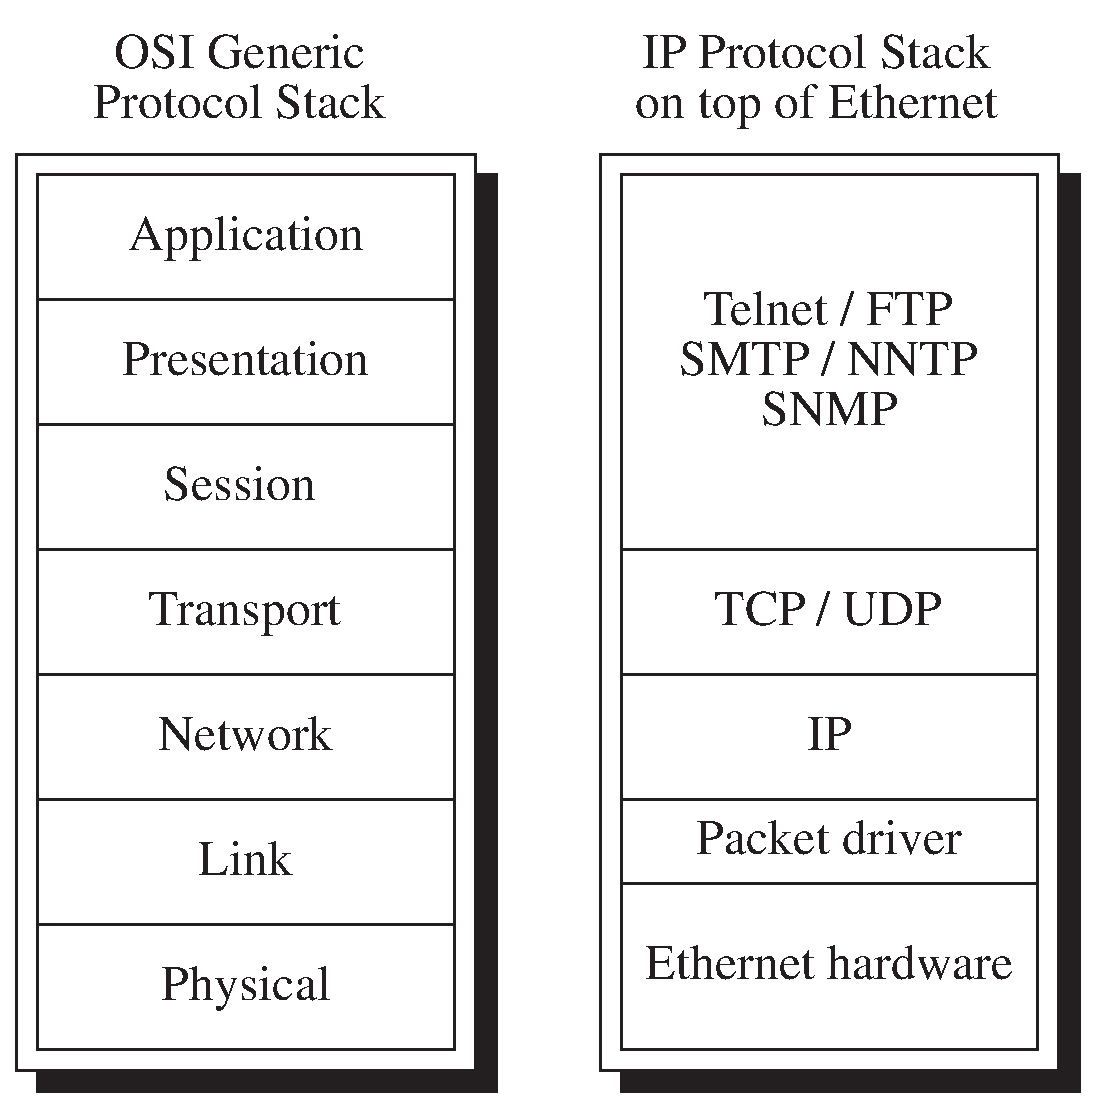
\includegraphics[height=3in]{pics/pstack}
\end{center}
\caption{OSI and TCP/IP Protocols Stacks}
\label{network:pstack}
\end{figure}

Throughout the history of computing there have been many network
protocols, most of them proprietary to specific systems.  As market
forces drive networks towards greater connectivity many of these
protocols have fallen by the wayside, leaving a handful of system
specific protocols and two major `open' systems.  Common network
protocols include SNA (Systems Network Architecture) from IBM, DECnet
from Digital Equipment Corporation, IPX (Netware) from Novell and
AppleTalk from Apple Computer.  The two major open systems protocols
are TCP/IP (Transmission Control Protocol / Internet Protocol) and OSI
(Open System Interconnection) (See Figure~\ref{network:pstack}).

\subsection{Internet Protocol}
\label{network:ip}

\subsubsection{History and comments}

The Internet Protocol, commonly known as IP, developed from ARPANET
(Advanced Research Project Agency NETwork), one of the earliest packet
switching networks developed \cite{RFC:791}.  ARPANET was funded by
the United States Department of Defence, who required a computer
network able to survive a limited nuclear attack.  For this reason
emphasis was placed on distributing decision making (as any
centralised system would be an obvious target) and reliability in
extreme circumstances.

ARPANET no longer exists but has been replaced by the {\em Internet},
a world wide network of networks, all using IP as their base
technology.  IP is a datagram protocol and is usable over a very wide
range of transmission technologies.

\subsubsection{Deployment within the University}

IP addresses are 32 bits wide and are split up into two parts, the
first being the network address and the other the host address.  IP
routes packets to the network level where it expects to be able to
communicate directly to the host.  Originally IP addresses were split
up into classes, for example class B addresses had 16 bits for the
network address and 16 bits for the host address, with class C having
24 bits for the network address and 8 bits for the host address.

The class of the address was encoded into the high bits of the address
so a router could tell how many bits it needed to make a routeing
decision on.  This fixing of the address part sizes was extremely
limiting so it was replaced by a 32 bit contiguous mask.  The mask
indicates which part of the address is the network part.

TCP/IP is deployed throughout the university and is available to all
departments.  Currently the university has a class B address which is
split up into 256 class C addresses using address masks.  This is
important for routeing packets within the university network.  From the
outside the university has a single 16 bit network address {\ttfamily
130.216.0.0} (the full address is always used even though the only the
top 16 bits are significant, non significant bits are set to zero) but
inside the university all networks addresses are 24 bits wide, for
example mathematics is {\ttfamily 130.216.15.0}.

\subsection{AppleTalk}
\label{network:appletalk}

\subsubsection{History and comments}

{\em AppleTalk} is the network protocol suite developed by Apple
Computer Inc. when it released the Macintosh \cite{AppleTalk:Apple}.
It was developed specifically for small local area networks.
Originally it only ran over {\em LocalTalk}, a bus topology physical
network.  LocalTalk has a very low bandwidth by today's standards but
it didn't require any extra hardware since all Macintoshes come with
it built in.  In later versions {\em EtherTalk} was added.  This
enabled the AppleTalk protocols to run over standard Ethernet.

It is mainly used for connecting Macintoshes to file servers and
printers.  Over small networks (up to the size of a campus network)
the protocol runs without difficulty.  It has a distributed directory
service which makes using it simple, but limitations in that protocol
now limit how large the network can grow.

AppleTalk cannot easily be used over wide area networks.  This is
mainly to do with limitations in its ability to address physical
entities on the network.  Also, the directory service breaks down over
slower links.

AppleTalk splits the network up into logical {\em zones}, where one or
more physical segment belongs to a zone.  Zones are not used in packet
routeing but are for human use only, dividing the network up logically
to simplify directory lookups, that is AppleTalk has a two level
directory consisting of zones and logical entities, which belong to
exactly one zone.  Because zones cannot belong to other zones,
connecting two separate AppleTalk networks, say two universities, is
infeasible without extreme care.

\subsubsection{Deployment within the University}

AppleTalk is also widely deployed throughout the campus.  The majority
of the network is over Ethernet with some outlying sections using
LocalTalk.

\subsection{IPX}
\label{network:ipx}

\subsubsection{History}

IPX, or {\em Internet Packet eXchange} is the network layer protocol
used by {\em Netware} \cite{Novell:IPX}.  Netware is a product from
Novell Inc which provides file server and remote printing services.  A
Netware network is a collection of file and printer servers connected
together using IPX.  Client machines, running MS-DOS or Windows,
connect to a server, and software on the client machine makes the
remote file systems behave as if they were connected locally.

IPX itself is a very simple protocol with a two level addressing
system.  Physical segments are each assigned an address, and machines
on the physical segments are addressed using their hardware address.
This simplicity reduces the amount of computing required to send each
packet, but limits the flexibility of the protocol.  IPX runs almost
exclusively over Ethernet.

\subsubsection{Deployment within the University}

IPX can go over any Ethernet segment provided it is able to be routed
onto it.  Most departments have enabled IPX routeing and often their
Novell servers also do IP and AppleTalk routeing.

Netware also places a non trivial load on the network because every
two minutes (or however long the administrator sets it) the router
broadcasts information about every Netware service available.  When
the number of file servers exceeds twenty this information becomes
large in size.  Currently the information is about 500 kilobytes in
size.  On busy networks such as student labs, this is unwelcome extra
traffic.

\section{Physical transmission media}

While the number of common network protocols is less than ten the
number of ways of transmitting digital information is at least five
times this.  Each method differs in behaviour and hence alters the
characteristics of traffic using it.  Fortunately most methods fall
into broadly defined groups, with each member of the group exhibiting
similar behaviour.

\subsection{Analog and digital transmission technologies}

All data transmitted is electro-magnetic energy at some stage (whether
it be light, radio or signals along copper wire) and as such is analog
in nature.  All modern data communication is digital in nature so
transmission requires signals to be encoded.  The term {\em bandwidth}
originally came from broadcasting, where it determined how large a
slice of the radio spectrum a transmitter could use.  This in turn
governed the frequency range of the transmission and how much
information could be sent in a given period of time.  The modern usage
still measures the rate at which data can be sent but unless specified
should not be seen as relating to the underlying analog technology.

\subsection{Point to point connections}

Point to point connections are the easiest to visualise.  {\em
Transceivers} (devices which both transmit and receive data) are
placed at either end of a cable.  If both transceivers can send
simultaneously then the medium is said to support {\em full duplex}
transmission otherwise the medium is said to be {\em half duplex}.

Point to point connections have two major characteristics.  The first is
bandwidth, measured in bits per second (bps) and in magnitudes of
multiples of one thousand (this is different from computers where
orders increase in multiples of $2^{10}$).  The other is {\em
latency}, which is a measure of delay between when data is sent and
subsequently received.  This is normally measured in the orders of
seconds (for example, milliseconds or microseconds).

\subsubsection{Framing}

Data is not sent in a raw stream but is encapsulated into discrete,
limited size packets, known as {\em frames}.  Framing the data avoids
excessive error propagation as well as providing information for
clock synchronisation.  Frames may also contain information about
addressing data to a particular transceiver and error correction.

Frame sizes vary from as little as 53 {\em octets} (an octet is eight
bits,  the term byte is normally used with respect to computers) to
over 8192 octets (8 Kbytes).  It is important for protocols using a
particular transmission medium to match their packet sizes to that of
the transmission frames.

\subsubsection{Serial and parallel connections}

Modern computers normally store data in blocks of 32 or 64 bits.  When
transmitting these blocks inside the computer they are sent in {\em
parallel}, that is to say 32 or 64 separate connections are used, with
each bit being sent simultaneously.  This means that large amounts of
information can be sent rapidly.

When sending data between two computers physical wires are required
making very wide parallel cables extremely expensive.  While eight bit
wide parallel cables are common they only ever extend a distance of
metres.  Wider cables are now being used to connect computers to high
speed peripherals but only up to a distance of one or two metres.

Over longer distances these blocks of data are sent bit by bit in
sequence.  This is known as {\em serial} transmission and only
requires two copper wires or one optical fibre per direction.  Over
any significant distance it is cheaper to make serial transmission
faster than to make parallel cables wider.

\subsection{Contention and bandwidth allocation}

When two or more parties attempt to simultaneously use a limited
resource then one or more must miss out.  This fighting is called {\em
contention} and the process for deciding who finally gets the resource
is called {\em contention resolution}.  Contention occurs in many
places in computing and specifically in data transmission where it is
associated with transmitters wanting to simultaneously send data with
limited bandwidth.

Contention can be resolved in a number of ways, each having advantages
and disadvantages.

\begin{itemize}

\item Stations are given set priorities.  If a station with a higher
priority wants to send then any sender which is lower must stop.  This
is called a {\em priority based} system.

\item A centralised station gives the right to send to subservient or
slave stations.  This is called {\em polling}.

\item The right to send is passed from station to station in an
orderly fashion.  This method is called {\em token passing}.

\item Two or more stations attempt to send and collide.  They then
fight among themselves until there is a winner who gets the right
to send.  These are called {\em contention} networks.

\item Data is transmitted in buckets and stations wanting to send must
let a certain number of empty buckets pass before they can use one.
This broadly falls into the category of {\em distributed queue}
networks.

\end{itemize}

\subsection{Broadcast media}

Radio, television and satellite are all broadcast media.  All
receiving stations get an identical signal from the sender.  This can
in principle be extended to include all receivers connected to a
single piece of wire.

This idea can be taken further and we may define a broadcast network
as a network such that any station can send a single packet to every
other connected station, which will receive an identical copy of that
packet.  This definition includes all physical topologies where
signals are propagated to every connected station.  Hence we can
include such networks as token ring and dual bus networks.

Broadcasting is very useful for sending information to every station
and is very efficient provided the transmission technology is based on
network wide signal propagation, where broadcast essentially comes for
free.  When the physical technology does not allow for broadcasting it
must be simulated.  This means every station wanting to receive
broadcasts must have the message individually sent to them.  For any
network of non trivial size this can become hugely expensive in
bandwidth.

\subsection{Common transmission technologies}

Below is a quick overview of common transmission technologies.  Full
details of some of them will be given in later chapters.

\subsubsection{Ethernet}

\begin{figure}
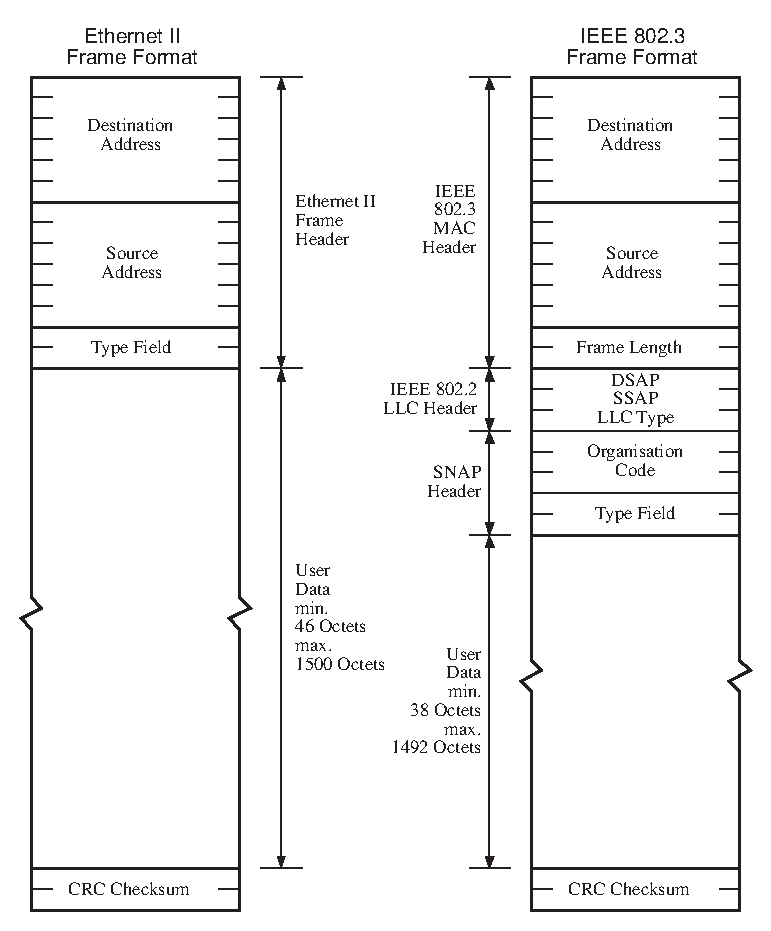
\includegraphics{pics/enet.eps}
\caption{Ethernet II and IEEE 802.3 Frames}
\label{network:enet}
\end{figure}

Ethernet is a contention based broadcast network designed to work over
short distances (tens to hundreds of metres).  It is the most widely
deployed transmission technology in computer networking with equipment
cheaply and widely available.  Its relative ease of installation and
maintenance has lead to it becoming the baseline technology within the
micro computer industry.  It is now known as IEEE 802.3, the standard
which currently defines it \cite{Digital:Ethernet}
\cite{IEEE:Ethernet}.  The raw transmission speed is normally 10 Mbps
but work is proceeding on defining a 100 Mbps standard.

The original Ethernet is now known as Ethernet II or Blue Blue
Ethernet, after the colour of the book which defined the standard.  It
is physically compatible with IEEE 802.3 but has a different frame
structure (See Figure~\ref{network:enet}).  Ethernet II is still
commonly used, especially with respect to TCP/IP.

\subsubsection{Token ring}

Token ring, specifically the standard IEEE 802.5, is a token passing
broadcast network \cite{IEEE:Tokenring}.  It is not as common as
Ethernet and is normally associated with IBM equipment.  Token ring
normally has a raw data rate of either 1, 4 or 16 Mbps.  Note that it
is unwise to make a direct comparison between these rates and that of
Ethernet as raw transmission rate is a poor indicator of true
throughput.

\subsubsection{FDDI}

FDDI, or Fibre Distributed Data Interface, is another token passing
network.  It is very similar to IEEE 802.5 except it runs on optical
fibre rather than copper wire.  Raw transmission rate (as seen by a
connected station) is 100 Mbps.

\subsubsection{PPP and SLIP}

While not physical technologies these define how data is to be sent
along serial connections.  SLIP (Serial Line Internet Protocol) is a
de-facto standard used because of its simplicity and wide availability
\cite{RFC:1055}.  PLIP (Parallel Line Internet Protocol) is an
analogous standard for parallel connections but is fairly uncommon.
PPP (Point to Point Protocol) is a full and complete standard for
transmitting packets over point to point connections \cite{RFC:1661}.
It provides Data Link layer functions such as error checking for the
link.

\section{The University campus network}

The campus network is a collection of physical networks connected
together via routers.  A majority of the physical networks are
Ethernet, either using copper wire or point to point connections using
optical fibre.

\begin{figure}
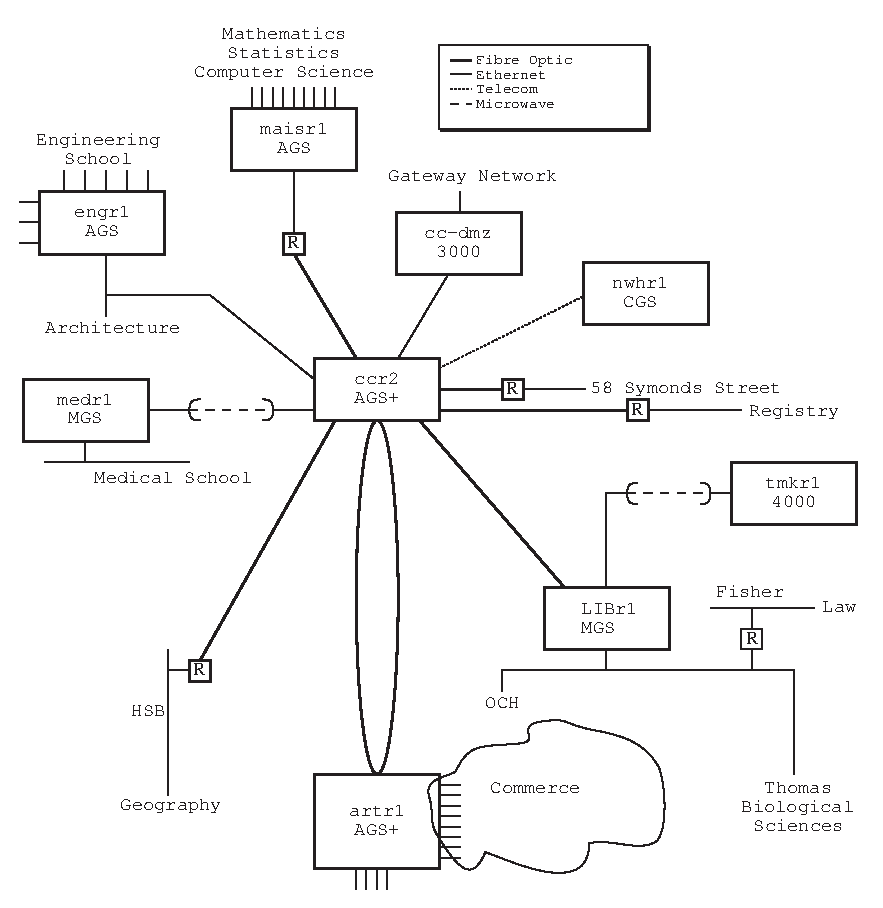
\includegraphics{pics/uni-network-map.eps}
\caption{Topological map of the University of Auckland Network}
\label{map:uni}
\end{figure}

\subsection{Computer Centre network}

\begin{figure}
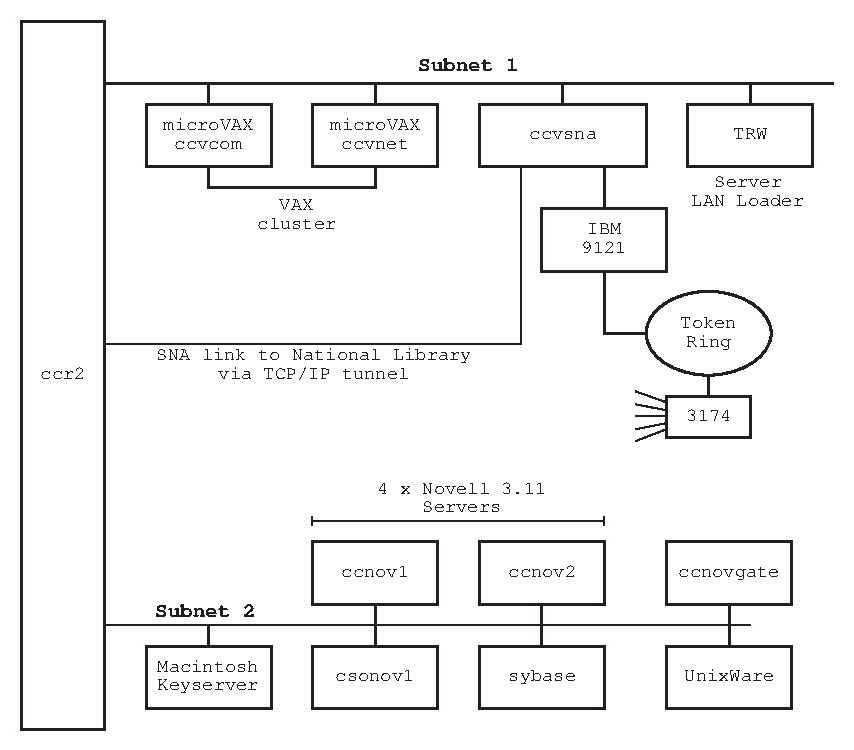
\includegraphics{pics/subnets-1-2-map.eps}
\caption{Topological map of part of the Computer Centre Network}
\label{map:ccnet}
\end{figure}

The computer centre network did have five sub-networks when the
experiments were being performed.  Since then a major re-arrangement
has taken place; this is not reflected here.

The network consisted of subnet 1, which connected the staff offices
and the VAX cluster, subnet 2, which held the computer centre Netware
servers and subnet 3 which had the Unix hosts.  There was also a
subnet 9 which served the terminal room containing PCs with Netware
and Macintoshes.

\subsection{Gateway network}

\begin{figure}
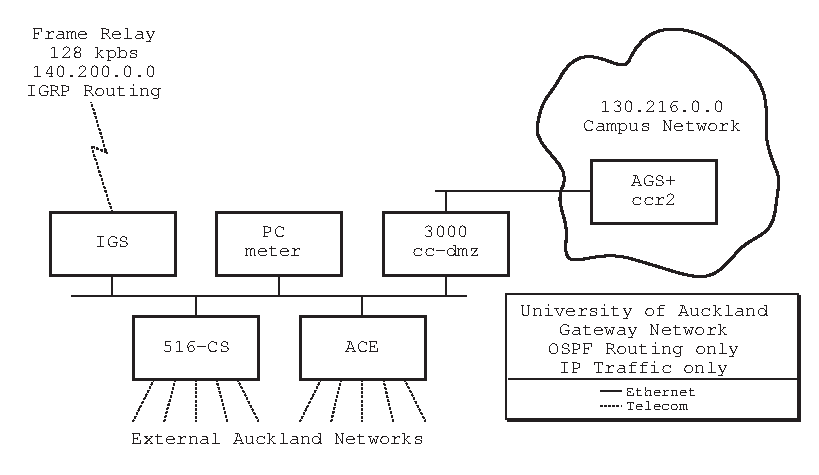
\includegraphics{pics/gateway-net-map.eps}
\caption{Topological map of the University Gateway Network}
\label{map:dmz}
\end{figure}

The gateway network, commonly known as the DMZ (Demilitarized Zone)
network, is used to separate the University network, the Auckland
local networks connected though common carrier dialup and leased
lines, and the frame relay connection to the rest of New Zealand and
the world.

\chapter{Network tracing}
\label{trace}

A network (or packet) {\em trace} is a record of activity of a
physical network over a period of time.  A network trace can contain
information about the length of each packet, the time it was seen and
part or all of the actual packet contents.

The emphasis of this thesis is traffic intensity with respect to time.
For this packet inter-arrival times are needed.  This is done by
recording a time-stamp in the trace.  The more accurate the time-stamp
the finer the analysis that can be performed.

For packet size analysis the length of the packet has to be recorded.
Because packet sizes are a function of higher level protocols, for any
in-depth analysis the origin of the packet has to be obtained.  This
can be done by examining the contents of each packet and extracting
the relevant information.  This is a time consuming task so it cannot
be done during the execution of the tracing program.  Instead the
first forty to fifty bytes of each packet is recorded for later
processing.

Packet traces are normally stored as large binary files.  Programs can
then examine these files and perform statistical analysis on the data.
Recording a trace over any reasonable length of time produces large
files, in the order of megabytes or tens of megabytes.

\section{Producing a packet trace}

The packet traces of Ethernet segment were collected using an IBM PC
directly connected to the Ethernet.  Because of the broadcast nature
of Ethernet it is easy to record all packets sent on the network.  The
program records a time-stamp, the packet size and the first $n$ bytes
of the packet, where $n$ is defined at compile time.

The number of packets the program records is set at compile time, and
normally ranges from ten thousand to half a million.  In a later version
of the program it should be possible to specify the number of minutes
the program is to run.

\subsection{Format of the trace file}

\begin{figure}
\begin{center}
\leavevmode
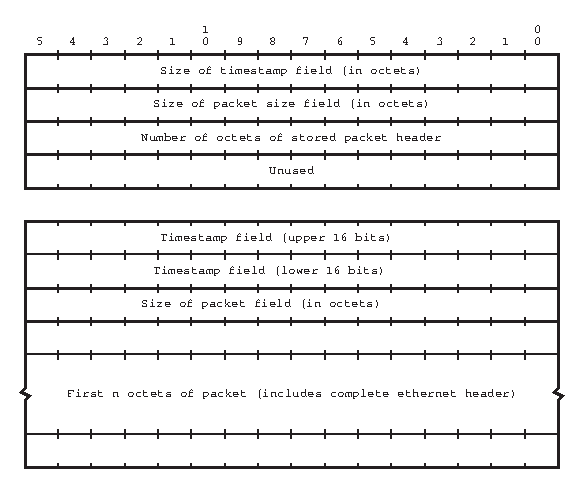
\includegraphics{pics/trace-format.eps}
\end{center}
\caption{Format of the trace file}
\label{trace:format}
\end{figure}

The trace file has an eight byte header containing four records, each
a two byte big endian word.  The contain the length of the time stamp
(in octets), the length of the packet size, the number of octets of
packet header and an unused word respectively (see
Figure~\ref{trace:format}).

Following the header are the actual trace records, which contain the
time stamp, the size of the packet (this includes the Ethernet header
but not the frame checksum) and the first $n$ octets of the
packet.

\subsection{Hardware used to produce the traces}

The hardware used was a standard IBM PC compatible with an Ethernet
controller.  This was used because it was easy to write the software
needed to produce the trace and because the hardware is widely, and
cheaply, available.  The IBM PC architecture does have several
drawbacks.

\begin{itemize}
\item	The clock used to generate the time stamps is limited in
accuracy to approximately 1 ms.

\item	The input/output bus is limited to transfers of about 700
kilobytes per second.  Very long bursts could be a problem.

\item	Interrupt events block other interrupts, causing problems
with the timer.
\end{itemize}

The Ethernet controller has an eight kilobyte buffer so as to reduce
the actual packet loses.  This may affect the analysis as queued
packets will be seen by the program as having a fixed inter arrival
time.

\subsection{Software used to generate the trace file}

The software is written in C and then compiled.  It is based on {\em
packet driver} software.  Packet drivers are pieces of code which
isolate the programmer from the specific details of each hardware
controller, presenting a standard interface regardless of the actual
controller.  This enables programmers to write much simpler programs
at the expense of a small extra overhead.

When a packet arrives at the Ethernet controller it generates a signal
to interrupt the processor and process the packet.  The packet driver,
while in interrupt mode (that is, the processor has suspended what it
was doing and is executing a special routine called an interrupt
handler) calls a user program with the size of the packet.  This
returns a pointer into memory for the contents of the packet to be
copied (this includes the packet header).  The driver copies the
packet and calls a second user program routine to tell it that the
copy has been completed.  Once the second routine has exited, the
packet driver then returns from interrupt mode, and the processor
restarts what it was originally doing.

The problem with interrupt mode is that code executing while in
interrupt mode cannot itself be interrupted (this is not strictly
correct but is true for packet drivers).  Interrupts which occur while
this happens are placed in a priority queue.  For this reason
interrupt handlers must do as little work as possible.  In general
programs just set flags and update simple data structures during
interrupt mode.

The program itself loops repeatedly checking these flags for change.
If a flag is set it then processes the packet from the head of the
data structure.  This looping is called {\em polling}.

\subsubsection{Data structures used}

The data structure consists of two fixed buffers.  While one is being
used the other is either waiting to be written out to a file or is
empty.  Each buffer has a fixed number of records into which packet
headers can be written.

The {\em Output File} is a standard C file pointer and is defined as
part of the C {\em stdio} (standard input/output) library.  This
enables the program to be portable to different operating systems.

There are also variables such as {\em Initial Time} and {\em Total
Packet Count} for determining when the program should terminate.

\subsubsection{Flow of polling loop}

\begin{figure}
\begin{center}
\leavevmode
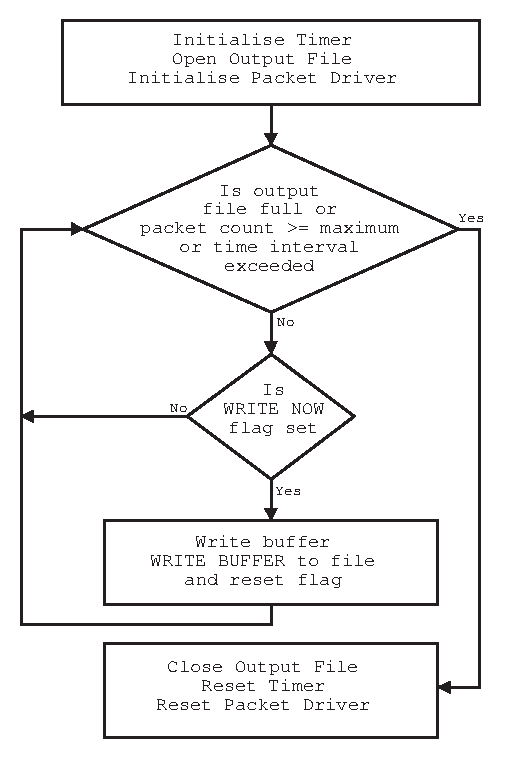
\includegraphics{pics/trace-flow.eps}
\end{center}
\caption{Flow of polling loop}
\label{trace:flow}
\end{figure}

The program has three stages.  The first initialises the required
variables and data structures, including the timer and packet driver.
The second is a repeated loop which continually checks to see if a
buffer needs to be written out to a file and the last is the final
clean up before exiting (Figure~\ref{trace:flow}).

There are various reasons for the program to terminate.  In the normal
course of events either the number of packets recorded reaches a set
amount or a running of the program exceeds a certain time limit.  Both
these values can be specified when the program is loaded into memory.
If the writing to the file should fail for some reason then the
program will also terminate.  Generally this will be because the disk
is full but other errors can occur.

\subsubsection{Flow during interrupt}

\begin{figure}
\begin{center}
\leavevmode
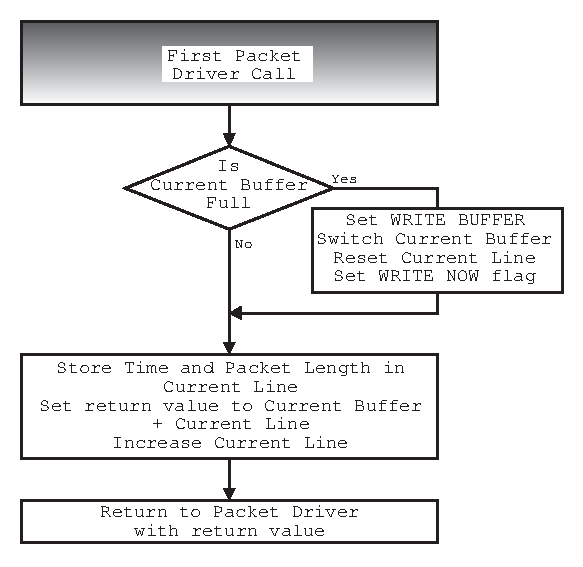
\includegraphics{pics/rcvPkt1-flow.eps}
\end{center}
\caption{Flow for first packet driver call}
\label{trace:rcvpkt1}
\end{figure}

\begin{figure}
\begin{center}
\leavevmode
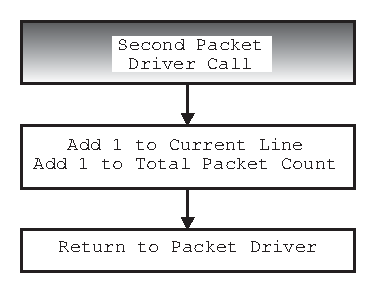
\includegraphics{pics/rcvPkt2-flow.eps}
\end{center}
\caption{Flow for second packet driver call}
\label{trace:rcvpkt2}
\end{figure}

When an interrupt is received by the packet driver it in turn calls
the user with the size of the packet and expects a pointer into memory
as a return result.  It also stores the current timer value and the
size of the packet into the current record
(Figure~\ref{trace:rcvpkt1}).

The packet driver then copies the contents of the packet into the
specified memory and calls a second user routine.  This simply updates
various counters and exits without any return value
(Figure~\ref{trace:rcvpkt2}).

\subsection{Known problems}

\subsubsection{Errors with the timer}
\label{trace:timerprob}

The timer works by having an internal 16 bit hardware counter, say
$c_0$. This starts at 0xFFFF (65535), counts down to 0x0000, then
resets itself automatically and starts counting down again.  When it
reaches 0x0002 it causes an interrupt and a counter $t$ kept by the
timer code is increased.  The counter is split into upper and lower
bytes, $c_u$ and $c_l$ respectively.  The value returned from the
timer is
\[
2^{8}t + (256 - c_u)
\]
which should theoretically always give the correct result.

The 1.19318 MHz clock generates the clock signals so that the standard
PC BIOS time is accurate to $\sim$ 18.2 Hz or 54.9 ms.  We use $c_u$
to give us a rate of 4.66 kHz or 0.2 ms.

Because the timer is asynchronous to the main processor, if $t$ should
fail to be increased at the correct time a problem may occur.  With
the Intel 80x86 processor a flag allows or blocks interrupts from
occurring.  If this flag is set then interrupts get queued, waiting
until the flag is cleared so they can occur.

If a packet arrives when $c$ is close to zero then an interrupt occurs
and the packet driver is called.  The packet driver sets the interrupt
flag (since another packet may be received while the driver is still
processing the first and if it was allowed to interrupt again the code
would probably crash).  While the driver is processing the interrupt
the timer reaches 0x0002, causes an interrupt, which is queued,
counts a little more and resets itself.

The tracing code then reads the value from the timer code, which is
now incorrect, since $t$ has not yet been incremented, and stores it
within the current buffer.  Afterwards the packet driver clears the
interrupt flags and exits, the timer interrupt occurs, $t$ is
incremented to the correct value, and the timer value is what it
should be.

The problem occurs because of a limitation of the Intel 80x86
architecture and cannot be avoided without considerable modification
of the packet driver code to stop it from having the interrupt flag
set while calling the user program code.  It is unclear whether this
is even feasible.

Because this problem is known it can be corrected in later processing
without much difficulty, so rather than try to fix it at
its origin it is simpler to make the corrections.

\subsubsection{Machine crashes after program exits}

After running the tracing program it is necessary to reboot the
machine it ran on.  This is more an inconvenience rather than a
problem.  The reason for the problem is unknown but the timer code is
the most suspect.  The amount of time needed to fix this problem is
not worthwhile and since it does not affect the results it can safely be
ignored.

\section{Testing the packet tracer}

\subsection{Introduction}

Having written this program a series of controlled experiments were
performed to check the validity and usefulness of the program.  Below
are some of the requirements of interest.

\begin{itemize}
\item	At what rate of packet arrival does packet loss occur?

\item	Does the size of the arriving packets affect packet loss?

\item	In what form does packet loss happen?

\item	How is packet loss affected by writing to permanent storage?
\end{itemize}

\subsection{Design}

This experiment was performed using two machines connected via an
isolated segment of Ethernet.  On one machine a packet generator
executes while the other records all packets seen on the segment and
writes them out to permanent storage.

One important note is the relative processing power of each machine.
While both machines have compatible architectures one is at least
twice as fast as the other.  This asymmetry enables the recording
program to be ``tested to destruction'' while the packet generating
machine remains stable.

The experiment was carried out by subjecting the recording machine to
various traffic loads (as specified by the generator's input
parameters) and examining the resulting output file.

\subsection{The packet generator}

The packet generator generates $c$ packets of fixed size $s$ octets.
Between the start of each packet is a delay $d$ ticks where a tick is
$\sim$ 0.2 ms.  If the time required to send a packet is greater than
the specified delay then the packets are sent end to end without any
artificial delay.  These three parameters can be specified on the
command line.

{\small
\begin{verbatim}
stress [-s packet size] [-c number of packets sent] [-c delay]
\end{verbatim}
}

$stress$ uses packet drivers for it communication with the Ethernet
hardware.  The code consists of a single loop which continually sends
out packets using the Ethernet broadcast address.  The current
sequence number and time follow the address within the packet.


\subsection{Experiment - determining the maximum output rate}

\begin{figure}
\leavevmode
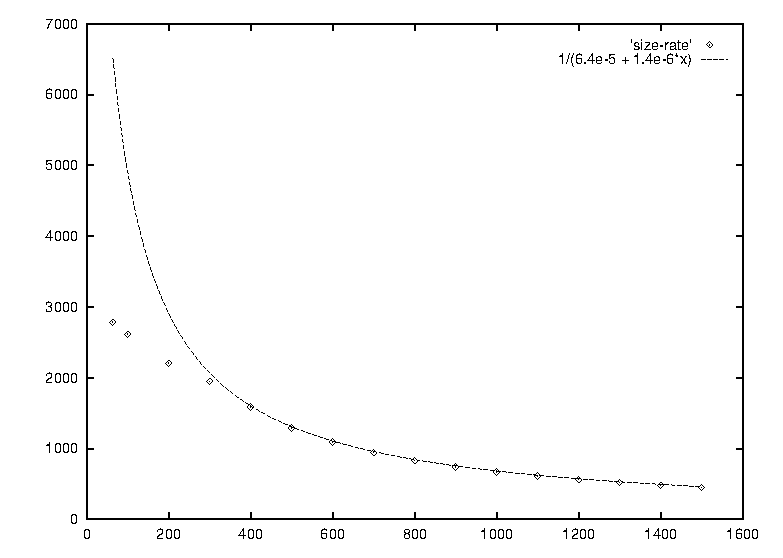
\includegraphics{pics/size-rate-fit.eps}
\caption{Output Rate versus Packet Size}
\label{trace:expr1}
\end{figure}

\begin{figure}
\leavevmode
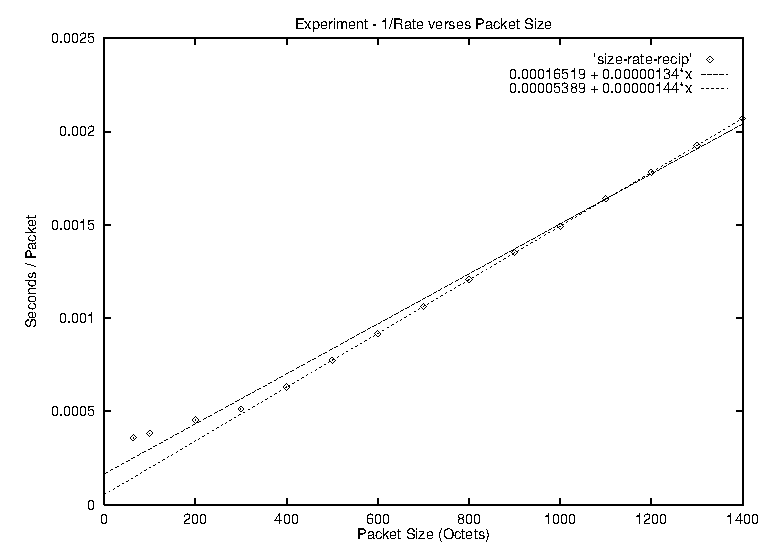
\includegraphics{pics/size-rate-recip.eps}
\caption{1 / Rate versus Packet Size}
\label{trace:expr3}
\end{figure}

\begin{table}
\begin{center}
\begin{tabular}{ccc}
{\bfseries Packet Size} & {\bfseries Packets per} & {\bfseries Octets per} \\
{\bfseries (octets)} & {\bfseries second} & {\bfseries second} \\
0064	& 2785 & 178240 \\
0100	& 2616 & 261600 \\
0200	& 2206 & 441200 \\
0300	& 1948 & 584400 \\
0400	& 1586 & 634400 \\
0500	& 1290 & 645000 \\
0600	& 1090 & 654000 \\
0700	& 0941 & 658700 \\
0800	& 0828 & 662400 \\
0900	& 0740 & 666000 \\
1000	& 0670 & 670000 \\
1100	& 0610 & 671000 \\
1200	& 0561 & 673200 \\
1300	& 0519 & 674700 \\
1400	& 0483 & 676200 \\
1500	& 0451 & 676500 \\
\end{tabular}
\end{center}
\caption{Results for maximum rate experiment}
\label{trace:expr2}
\end{table}

To examine the behaviour of the packet generator a series of packet
generations was carried out from the slower to the faster machine.
The experiment looked at the maximum rate (in packets per second) the
generator could produce given a specific packet size.  The result can
be seen in figures \ref{trace:expr1} and \ref{trace:expr3}, and
table~\ref{trace:expr2}.

These were produced by sending 10,000 packets back to back without
delay between the two machines.  The trace file is then analysed and
the number of packets per second is extracted using {\ttfamily arrival}.

The curve on figure \ref{trace:expr1} was produced by taking the
resulting values (table~\ref{trace:expr2}, ignoring the first four
values, taking the reciprocal and fitting a linear line to it.  In
figure~\ref{trace:expr3} you can see both line fits, one including all
the points and the other excluding the first four points.  This linear
fit was then inverted and plotted against the original points.

The results suggest that beyond packet sizes of 400 octets the
generator's output is bounded by the I/O (Input / Output) of the
machine, at about 710,000 octets/second or 693 K per second.  Packet
sizes smaller than this are bounded by the processing time needed to
send each packet so that the curve represents the maximum theoretical
output in packets per second.

Note that 710,000 octets/second is less than Ethernet's theoretical
throughput of around 1,200,000 octets/second so that on a faster
machine with greater I/O bandwidth more than 700 K per second is
easily achievable.

\subsection{Summary of packet trace test}

\begin{itemize}

\item
No losses were observed in the experiment, and th packet rates used
there are higher than those observed on the Campus network.

\item
In the experiment there was on evidence of packet loss during writes
of the trace data to disk storage.

\end{itemize}

Overall the trace program performed very well, providing a simple and
effective tool for collecting network traffic data.

\chapter{Stochastic Models of Packet Arrivals}
\label{models}

To simulate packet arrivals we must first define models of packet
arrivals.  Most of the early work in this area used the Poisson
process \cite{grimmett} as the basis of its models.  Many more complex
models have been used but many rely on the Poisson process somewhere
for the packet arrival distribution.  The Poisson process has the
advantage of being well understood and mathematically tractable.


The Poisson process is related to the exponential distribution (\S
\ref{append:expon}).  This distribution is one of the most widely
used in statistics and the basis for several others.  One feature of
the distribution is it has a finite mean and variance (\S
\ref{append:moments}).  The exponential distribution has the property
that the time spent waiting for an event (that will occur within a
time that is exponentially distributed) will not give you any
information about when it will occur.  This is known as the {\em
memoryless} property of the exponential (and its discrete counterpart
the geometric) distribution.

One important area of interest are processes which have inter-renewal
times with infinite moments.  We are mainly interested in those
distributions with infinite variance such as Cauchy,
$\mbox{t}_2\mbox{-distribution}$ and Pareto.

The research into infinite variance distribution renewal processes has
led to the idea of {\em fractal}, or {\em self similar} renewal
processes.  The basis of these names has to do with similar behaviour
at different time scales.  Poisson processes become smoother as you
observe their average behaviour over longer time intervals.  Pure
fractal processes do not smoothe so that they are invariant with
respect to the time period over which you observe them.

Such behaviour has serious consequences when applied to traffic models
because it indicates that you will always get bursts of traffic at
every time scale and you can never allocate enough queueing resources
to cope with every situation.

Much of the original work into fractals was done by Mandelbrot
\cite{IEEE:Mandelbrot} but it is only recently that his work has been
applied to communications traffic by researchers at Bellcore
\cite{Bell:1},\cite{Bell:2}, \cite{Bell:3}, \cite{Bell:4}.

The use of finite variance distributions was challenged in
\cite{Bell:1}.  In this thesis we examine the behaviour of Poisson
process based models and demonstrate that they are inadequate for
modelling network traffic observed on the University of Auckland
campus network.

The researchers at Bellcore produced traces for Ethernet LAN traffic,
ISDN packet traffic over public switched telephone systems and the
output of variable bit rate video encoders.  The earlier chapters of
this thesis attempted to duplicate their recording of Ethernet traffic
and produce comparable results as confirmation of their work.

The Bellcore work then went on to examine many of the self-similar
properties of the traffic and its relationship to theoretical work in
fractal behaviour.  In this thesis we simulate various statistical
models to see whether the observed behaviour can be reproduced.

\section{Poisson process}

\subsection{Definition}

A Poisson process is a counting process
\[ N = \{ N(t) : t \geq 0 \} \]
taking values from
\[ S = \{ 0,1,2,3, \ldots \} \]
conditioned on
\[N(0) = 0\]
and
\[ \mbox{if } s < t \mbox{ then } N(s) \leq N(t) \; \forall s,t \in {\mathbb R} \]
defined by
\[
\begin{array}{c}
P(N(t+h) = n + m | N(t) = n) = \\
P(N(t+h) - N(t) = m) = \\
\left\{
\begin{array}{rl}
1 - \lambda h + o(h) & m = 0 \\
\lambda h + o(h) & m = 1 \\
o(h) & m > 1 \\
\end{array}
\right. \\
\end{array}
\]

\subsection{Remarks}

The Poisson Process is one of the most common and simple stochastic
processes in statistics and operations research.  Poisson processes
occur in both time and space and are characterised by a single
parameter $\lambda$.  This parameter $\lambda$ is a measure of the
rate or intensity of the process.

Poisson processes in time occur along a real valued time line,
normally ${\mathbb R}^+$.  They create single events along the line as they
advance towards $+\infty$.

The above definition has the following consequences.

\begin{itemize}
\item	No event may occur at exactly time zero.

\item	The numbers of events in two non-overlapping time periods are
independent.  For example knowing the number of events in the period
$(0, t]$ will not give you any extra information about the number of
events in the period $(t, t+s]$, that is $N(t+s) - N(t) \sim N(s) \;
\forall s,t \in {\mathbb R}^+$.

\item	The number of events in the period $(0, t]$ is distributed
as a Poisson$(\lambda t)$ random variable, that is $P(N(t) = x) =
\frac{e^{-\lambda t}{\lambda t}^x}{x!}$, independently of all other
inter-event times.

\end{itemize}

It can easily be shown that these give us the following.

\begin{itemize}
\item	The time between any two successive events is distributed
$\mbox{Exponential}(\lambda)$, that is $P(T_i - T_{i-1} \geq t) =
e^{-\lambda t}$.

\end{itemize}

\section{Renewal processes}

A renewal process can be seen as a generalisation of a Poisson
process.  The distribution of the times between renewal events are
independent and identically distributed random variables.  For example
the Poisson process is a renewal process because the inter-arrival
times are independent and identically distributed (as exponentially
distributed random variables).  Renewal processes periodically
restart themselves at the renewal points, forgetting their previous
history.

The behaviour between renewal events may be complex.  Often the
renewal event is a marked event within a more complex process.  An
example is the simple random walk where the return to the origin or
return to zero can be used as the renewal event.  This is to maintain
consistency with the concept that when a renewal occurs it is as if
the process were starting from time zero.

\subsection{Simple renewal processes}

\subsection{Definition}

Let
\[ T = \{T(k) : k \geq 0 \; k \in {\mathbb N} \} \]
where $T(k)$ is the time of the $k^{th}$ event, conditioned on
\[ T(0) = 0 \]
Let
\[ \begin{array}{c}
R_k = T(k) - T(k-1) \\
R_k > 0 \; \;  k \geq 1 \\
\end{array}
\]
Then this is a renewal process if there exists a
distribution function $F_R(x)$ such that

\[ P(R_k \leq x) = P(R \leq x) = F_R(x) \; \forall x > 0 \mbox{ and } \forall k\geq 1 \]
Furthermore, the $R_k$ are mutually independent of one another.  That
is, inter-event times are independent and identically distributed.

\subsection{Remarks}

In simple renewal processes the process restarts every time an event
occurs.  This is the simplest type of renewal process and is very
similar to the Poisson process.  The main difference is that the
Poisson process relies on events having an exponentially distributed
inter-arrival time.  In a renewal process any probability distribution
may be used for the time until the next renewal.

Because the time until the next renewal has to be non negative
many common distributions such as the normal or Cauchy have to be
modified.  This can be done by folding the negative half of the
density onto the positive real line.  The simplest method is sampling
from the distribution and then taking the absolute value.

\subsection{Processes with internal structure}

Many processes are more complex then single events.  Between renewals
the process may produce other events.  A M/M/1 queue is a simple
queueing process where the time between arrivals is exponentially
distributed and the time taken for the customer at the head of the
queue to be served and leave is also exponentially distributed.  We
can make the renewal event the event of the system becoming empty.
The times when the system becomes empty form a renewal process with
the queueing process becoming hidden.

\section{Modulated processes}

Modulated processes are multi-state stochastic processes.  They
consist of individual states and a set of stochastic transitions which
govern the process' change from one state to another.

The process is in exactly one of the states at any given time.  While
it is in a state it acts in accordance with the behaviour that state
specifies.  The process may change state at any time and must enter
another state straight away.  The rules governing how long the process
stays in a state and which states can follow it may be state dependent
or be controlled by an underlying global process.

The difference between modulated processes and renewal process is that
each state in the modulated process has an associated renewal process
which produces events.  When a new state is entered a new renewal
process corresponding to that state is created rather than each
renewal process continuing to run but being hidden, producing events
which are then discarded.

For Markov modulated Poisson processes there is no difference because
of the memoryless property of the exponential distribution but for
more general processes this distinction is important.  This is due to
the {\em edge effects} created by the renewal process creation at
state changes.  If the lifetimes for the states are short causing
rapid state changing then these edge effects may seriously affect the
overall behaviour of the process.

\subsection{Markov modulated Poisson processes}

\subsubsection{Definition}

Let

\[ \mathcal{S} = \{s : s = 0,1,2,3,\ldots, N \} \]

be a set of states with associated arrival rates $\lambda_s$, where
$\lambda_s$ is the arrival rate of the underlying Poisson process
while in state $s$.  Let

\[ N = \{ N(t) : t \geq 0 \} \]

be the underlying Poisson process of rate $\lambda_{S(t)}$.  Let

\[
S = \{ S(t) : S(t) = s \in \mathcal{S} \; \; \forall t \geq 0 \; \; t \in {\mathbb R} \}
\]

be the state of the process at time $t$.  Let

\[
P(S(t+\delta) = k, \; 0 < \delta \leq h | S(t) = k) =
e^{- \mu_k h}
\]
where $\mu_k \in {\mathbb R}^+$ are state lifetime parameters, with
\[
\begin{array}{c}
P(S(t+h) = k | S(t) = j, h = \mbox{inf}\{S(t + \delta) \neq j \;,
\delta > 0\}) = M[j,k] \; \forall j,k \in {\mathcal S}, \\
M = M[m,n] \\
\end{array}
\]
is a stochastic $|\mathcal S| \times |\mathcal S|$ matrix such that
\[
\sum_n M[m,n] = 1 \; \; \forall m \in {\mathcal S}
\]

\subsubsection{Remarks}

Markov modulated Poisson processes are the simplest of the modulated
processes.  Each state defines the arrival rate of an underlying
Poisson process.

The amount of time the process stays in a state is exponentially
distributed with a stochastic transition matrix governing the next
state entered.

Markov modulated Poisson processes are often used to generate the
arrivals for standard queueing models.  This is so that more
variability is introduced into the model and to add extra realism
rather than having a constant arrival rate.

\subsection{Generalised modulated processes}
\label{models:genmodproc}

\subsubsection{Definition}

Let
\[ {\mathcal S} = \{s : s = 0,1,2,3,\ldots, N \} \]
be a set of state with associated distribution functions
\[
L_s : (0, +\infty) \rightarrow [0,1] \; s \in {\mathcal S}
\]
Let
\[
S = \{ S(t) : S(t) = s \in {\mathcal S} \; \; \forall t \geq 0 \; \; t \in {\mathbb R} \}
\]
be the state of the process at time $t$, $c(t)$ be the number of state
changes by time $t$, $\sigma \in {\mathcal S}$ be a starting state $S(0) =
\sigma$ and $\tau_n$ be the time of the $n^{th}$ change of state.
\[
\begin{array}{rcl}
\tau_0 & = & 0 \\
\tau_{n+1} & = & \mbox{inf}\{t : t > \tau_n, S(t) \neq S(\tau_n) \} \\
\\
c(t) = n & \mbox{iff} & \tau_n  \leq t \mbox{ and } \tau_{n+1} > t \\
\end{array}
\]
Let
\[ N_i = \{N_i(t) | N_i(0) = 0 \} \]
be a collection of simple renewal processes where $N_i(t) = k$ if $k$
events have occurred by time $(0,t]$ and $i \in {\mathcal S}$.  These are
template renewal processes.

Let
\[
P(\tau_{\alpha + 1} - \tau_\alpha > h) = 1 - L_{S(\tau_\alpha)}(h)
\]
with
\[
P(S(\tau_{\alpha + 1}) = k \;| \; S(\tau_\alpha) = j) = M[j,k] \; \forall j,k \in {\mathcal S}
\]
where
\[
M = M[m,n] \; \; 0 \leq m , n \leq |{\mathcal S}|
\]
is a stochastic matrix such that
\[
\sum_n M[m,n] = 1 \; \;  m \in {\mathcal S}.
\]
Let the current renewal process at time $t$ be
\[
Q_\alpha = \{Q_\alpha(t) \;| \; Q_\alpha(\tau_\alpha) = 0\} \mbox{ where } \tau_{\alpha} \leq t < \tau_{\alpha + 1}
\]
where
\[
P(Q_{\alpha}(t) = k) = P(N_{S(t)}(t - \tau_\alpha) = k)
\]
so that the total number of events by time $t$ is given by
\[
R(t) = \sum^{c(t)-1}_{i=0}{Q_i(\tau_{i+1})} + Q_{c(t)}(t)
\]
\subsubsection{Remarks}

A generalised modulated process consists of a set of states and a
stochastic transition matrix but unlike the Markov modulated Poisson
process it is not limited to only using the exponential distribution
as a lifetime distribution.

Each state has two distributions associated with it.  One is a renewal
process which generates events and the other is a lifetime
distribution.  When the process enters the state a lifetime is
generated from the lifetime distribution.  The process will remain in
that state for the period of the lifetime.

While in that state a renewal process will run generating events.  If
an event is generated which would have occured beyond the lifetime of
the state then it is ignored.  Any generalised renewal process is able
to run provided it is independent of all other states.

Once the lifetime of a state has expired then the process chooses a new
state to enter based on the probabilities in the transition matrix.
The transition matrix is constant and independent of any activity
within any of the states.

\section{Merged Processes}
\label{models:mergedprocs}

\subsection{Definition}

Let
\[ {\mathcal C} = \{c:c = 0,1,2,3,\ldots, N\} \]
be a set with associated general renewal processes
\[R_c(t), \; c \in {\mathcal C} \]

Let
\[ T_c = \left< T_{c_1}, T_{c_2}, \ldots \right> \]
 be the sequence of renewal times of the process $R_c$.

Let 
\[ T = \left<T_1, T_2, T_3, \ldots \right> = \bigcup^{\mathcal C}T_c \]
 be an ordered sequence such that 
\[ T_i \leq T_j \; \forall i,k \in {\mathbb N} \]
then T is a merged process.

\subsection{Remarks}

A merged process consists of multiple renewal or modulated processes
running concurrently with their resulting event traces merged
together.  In most models each process is identical and all must be
mutually independent.

The idea behind merged (or superimposed) processes is to capture
complex behaviour using simply renewal processes with few parameters.
This would give us a much simpler model without losing the complex
nature of the real behaviour.

\section{Slowly decaying variances}

\subsection{Processes with infinite moments}

There are several well known distributions with infinite moments.  The
t-distribution has infinite variance for $\nu = 2$ and infinite mean
and variance for $\nu = 1$ (this is also known as the Cauchy
distribution).  Another is the Pareto distribution.  This is a less
common distribution and is not often used in the area of stochastic
process modelling.

\subsubsection{Definition of the Pareto distribution}

\[
F_X(x) = P(X \leq x) = 1 - \frac{\beta^\alpha}{(\beta + x)^\alpha}
\]
and
\[
f_X(x) = \frac{\alpha \beta}{(\beta + x)^{\alpha + 1}}
\]
so that $\alpha = 2.5$ with give a distribution with finite mean and
variance, $\alpha = 1.5$ will give infinite variance and $\alpha =
0.5$ will have both infinite mean and variance.

\subsection{Aggregating stochastic processes}
\label{models:aggregation}

One of the methods for testing whether a sample has been generated
from a Poisson process is to see how the variance behaves under
averaged aggregation \cite{Bell:5}.

Let
\[
X = (X_1, X_2, X_3, \ldots)
\]
be a stationary stochastic process (for us $X_k$ will denote the
number of events per time unit).  For each $m = 1,2,3,\dots$ let
\[
X^{(m)} = (X^{(m)}_k : k = 1,2,3,\ldots) 
\]
denote a new (aggregated) time series obtained by averaging the original
series $X$ over non-overlapping blocks of size $m$.  That is for $m =
1,2,3,\ldots$, $X^{(m)}$ is given by
\begin{equation}
X^{(m)}_k = \frac{1}{m}(X_{km - m + 1} + \cdots + X_{km}) \; (k = 1,2,3,\ldots)
\label{models:eq1}
\end{equation}
Note that $X^{(m)}$ defines a new stationary process for each $m$.
 

Consider any collection of random variables which have the following
properties

\begin{itemize}

\item	All variables are independent and identically distributed.

\item	Their probability distribution have finite mean $\mu$ and
variance $\sigma^2 \in {\mathbb R}^+$.

\end{itemize}

Let
\[
X = (X_1,X_2,\dots,X_n)
\]
and
\[
{\bar X} = \sum^n_{i=1}\frac{X_i}{n} = \frac{1}{n}\sum^n_{i=1}X_i
\]
then
\[
\mu_{\bar X} = \mbox{E}({\bar X}) = \mbox{E}( \frac{1}{n}\sum^n_{i=1}X_i)
= \frac{1}{n}\sum^n_{i=1}\mbox{E}(X_i) = \mu
\]
and
\[
\sigma^2_{\bar X} = \mbox{Var}({\bar X}) = \mbox{Var}(\frac{1}{n}\sum^n_{i=1}X_i) = \frac{1}{n^2}\sum^n_{i=1}\mbox{Var}(X_i) = \frac{\sigma^2}{n}
\]

From above we can see that for aggregated renewal processes with finite
mean and variance the variance is of order $n^{-1}$ under
averaging.  The decreasing of variance is called {\em decaying
variance}.  So from equation~\ref{models:eq1} we obtain

\begin{equation}
\mbox{Var}(X^{(m)}) \sim a_1 m^{-1}, \mbox{ as } m \rightarrow \infty
\end{equation}

With {\em slowly decaying variance} we do not get this, instead we observe
\begin{equation}
\mbox{Var}(X^{(m)}) \sim a_2 m^{-\beta}, 0 < \beta < 1 \mbox{ as } m \rightarrow \infty
\label{models:eq3}
\end{equation}

For summation $n{\bar X} = \sum^n_{i = 1}X_i$ we get $u_{n{\bar X}} = n
\lambda t$ and $\sigma^2_{n {\bar X}} = n \lambda t$.  This result
states for the aggregated random variables both mean and variance
increase linearly under summation.  For processes that exhibit slowly
decaying variance the result is that their variance grows faster than
linearly.  For a full example see \S~\ref{appendix:example1}.

Therefore to see the behaviour in equation~\ref{models:eq3} one or
both of the above conditions must fail to hold.  For any renewal
process the random variables will always be identically distributed
leaving either the distribution to have infinite variance and/or there
to be some dependence between the variables.

\section{Fixed interval counting}

Let
\[ T = \{T(k) : k \geq 0 \; k \in {\mathbb N} \} \]
where $T(k)$ is the time of the $k^{th}$ event, conditioned on
\[ T(0) = 0 \]
Let
\[ \begin{array}{c}
R_k = T(k) - T(k-1) \\
R_k > 0 \; \;  k \geq 1 \\
\end{array}
\]
Then this is a renewal process if and only if there exists a
distribution function $F_R(x)$ such that

\[ P(R_k \leq x) = P(R \leq x) = F_R(x) \; \forall x > 0 \mbox{ and } \forall k\geq 1 \]
and the $R_k$ are mutually independent.  That is, inter-event times
are independent and identically distributed.

Let
\[{\mathcal I} = \{i_k : i_k = [ks,(k+1)s) , k \in {\mathbb N} \cup \{0\}\} \]
be a set of non overlapping intervals of size $s$ such that $\cup
{\mathcal I} = {\mathbb R}^+$.

Let
\[{\mathcal C} = \{C_k : C_k = \{ j : T(j) \in i_k \} \} \]
so that
\[
c_k = |C_k|, k \in \{ 0,1,2,\ldots \}
\]
be the number of events in the interval $i_k$, that is $(ks, (k+1)s]$.

Then
\[
P(c_i = k, c_{i-1} = j) = P(c_i = k) \cdot P(c_{i-1} = j), i > 0
\]
is true $\forall s$ if and only if $T$ is a Poisson process.  That is for
general renewal processes $c_i, c_{i-1}$ are not independent.

For example, if we have a renewal process with inter-renewal events
distributed uniformly with mean 0.75, and a counting interval of
length 1.0 then for any interval $c_k$ where the previous interval
$c_{k-1}$ had no events must have at least 1 event in it.

This is because a uniform inter-renewal distribution with mean 0.75
has a maximum inter-renewal time of 1.5.  Since the previous interval
did not have any events ($c_{k-1} = 0$) in it then 1.0 of the maximum
of 1.5 has already occurred.  This means that event must occur within
the current interval ($c_k > 0$).  Hence the number of events that can
occur in the current interval is dependent on the number that occurred
in the previous interval, so the $c_{k-1}$ and $c_k$ are no
independent.

\chapter{Experimental Results}
\label{results}

\section{Introduction}

In this chapter the we examine four samples from around the University
(See Table~\ref{results:sampletable}), taken over a period of five
months during 1994.  The results are displayed as graphs along with
commentary about any notable features.  There are also notes on how
the graphs were obtained and any interesting results.

The samples have been taken from quite different environments to try
to give a wide selection of network protocols and traffic conditions.
Along with the results of the four samples, one of the samples has
been split up by network protocol.  The question of how each different
protocol affects the traffic behaviour is one this thesis would like
to try to answer, or at least gauge the basic similarities and
differences between the protocols.

\begin{table}
{\small \begin{tabular}{|l|l|l|l|l|l|} \hline
Date & Location & Traffic Mix & Load & Time & Packet Count \\ \hline \hline
14 May & Computer Centre & AppleTalk, Telnet & Heavy & 14 minutes & 400,021 \\
 & Staff Network & Novell client & & & \\ \hline
13 June & Gateway to & Various IP & Light & 102 minutes & 329,379 \\
 & Outside World & & & & \\ \hline 
1 August & Statistics & IP, mainly NFS & Light & 118 minutes & 400,048 \\
 & & & & & \\ \hline
1 September & Commerce & NetBIOS from & Medium & 94 minutes & 800,002 \\
 & & Windows NT & & & \\ \hline
\end{tabular}}
\caption{Traffic Samples from around The University of Auckland}
\label{results:sampletable}
\end{table}

\section{Processing trace files}

Once the trace file has been recorded it is transfered to a Unix host
where it is processed.  The first processing done corrects the timer
problem (Section~\ref{trace:timerprob}).  The file may then be divided
up, based on the various protocols embedded in the packet, and used to
generate packet frequency (by time interval) data.

\subsection{Correcting the timer problem}

The correcting of the timer problem is a simple process.  Because the
timer error causes a time to be out by 256, by keeping some notion of
the minimum correct time we can determine whether a time-stamp is
earlier than it should be.  Adding 256 to the value corrects the
time-stamp to the right value.  This is done by the program

{\ttfamily \small \begin{flushleft}
  correct filename[.icr]
\end{flushleft}}
which produces a new file called {\ttfamily {\em filename}.tra}.  {\ttfamily
correct} also changes the time from ticks ($\sim 4648$ ticks per
second) to milliseconds.  This greatly simplifies all calculations and
removes any dependence on the PC timers.

\subsection{Producing frequency data}

The process of producing discrete time interval packet and octet
counts is very simple.  The program {\ttfamily arrival} is given the slot
size in milliseconds and told whether the output should be a binary
file or an ASCII text file.

{\ttfamily \small \begin{flushleft}
  arrival [-b binary] [-t interval time] filename[.tra]
\end{flushleft}}

\begin{figure}[t]
\begin{center}
{\ttfamily
\begin{tabular}{ccc}
4649	& 65	& 11524 \\
4650	& 66	& 12652 \\
4651	& 61	& 12261 \\
4652	& 56	& 10319 \\
4653	& 54	& 12231 \\
4654	& 57	& 10219 \\
4655	& 58	& 10704 \\
4656	& 66	& 12109 \\
4657	& 49	& 10574 \\
4658	& 60	& 11231 \\
4659	& 49	& 10424 \\
\end{tabular}}
\end{center}
\caption{Sample output of {\em arrival}}
\label{interval:figure1}
\end{figure}

The text output of {\ttfamily arrival} can be seen in
Figure~\ref{interval:figure1}.  The first column is the interval
number, the second the packet count and the third the total number of
octets.  The binary output has the same format except that the entries
are stored as 32 bit integer values.  The binary file also has the
total number of rows and columns stored at the end of the file as 32
bit integer values.  This is to help programs which read the file.

\subsection{Dividing trace into protocols}

To provide information on individual protocols packet traces need to
be separated.  This is done by a program {\ttfamily demux} (for
demultiplex), which takes each packet header in turn, analyses it and
decides via a set of rules which output file to store it in.

Currently the rules provide for IP, AppleTalk, IPX and most of DECnet.
As IP, IPX and AppleTalk make up the bulk of all the University's
network traffic this is adequate.

\subsection{Producing the histograms}

The histograms (figures \ref{results:snet1.1s.hist},
\ref{results:snet93.1s.hist}, \ref{results:gatew.1s.hist}, \ldots) were
produced using the following program:

{\ttfamily \small \begin{flushleft} hist [-w width] [-s smooth] filename[.tra]
\end{flushleft}}

{\ttfamily hist} reads in the files created by {\ttfamily arrival} and produces a
frequency histogram table.  As the input is packets per time unit
(normally one second) this gives us an indication of how the traffic
levels are spread.  This table is stored as ASCII so it can be
directly plotted.  To get around the problem of too much detail an
aggregation (smoothing) feature was added.  This takes the histogram
results and at successive intervals of size $s$ it sums the frequency
values, and outputs a single value for the interval at the average of the
corresponding packets per second.

\subsection{Producing slowly decaying variance results}
\label{results:stat}

To produce the slowly decay variance results the output from {\ttfamily
arrival} has to be processed.  This is done using the program

{\ttfamily \small \begin{flushleft}
  stat [-l logarithmic output] [-v verbose] [-m maximum] filename[.abf] ... \\
\end{flushleft}}
which automatically detects whether the file is text or binary and
reads it all into memory.  From the input file it builds up a vector
$\vec{u}$ in memory containing all the packet count values, say $size$
long.  Let the command line maximum be stored as $cmdmax$.

It then loops from $1$ to $\mbox{min}(size / 100, cmdmax)$ using the
variable $k$.  Let 
\[
\vec{v}_{k} \mbox{ be vectors of length } k
\]
 such that
\[
\vec{v}_{k_l} = \sum^{k \cdot (l+1) - 1}_{i = k \cdot l}{\vec{u}_i} / k
\mbox{ where } l \in \{0, \ldots, size \mbox{ div } k - 1\} \subset{\mathbb N}
\]

Let $var_k$ be the sample variance of the vector $\vec{v}_k$.  The
output file {\ttfamily {\em filename}.sta} is the textual representation of
the ordered pairs $(k, var_k)$.  If the {\ttfamily -l} command flag is
present then another file called {\ttfamily {\em filename}.dat} is also
produced with the ordered pairs $(\log_{10} k, \log_{10} var_k)$.

\section{Mean and standard deviation of samples}

\begin{table}[t]
\begin{center}
{\begin{tabular}{|p{4cm}|r|r|r|} \hline
Sample & Interval & Mean & Std. Dev \\ \hline \hline
Gateway Network & 10s	& 537.50 &  115.33 \\
		& 1s    &  53.70 &   17.48 \\
		& 100ms &   5.37 &    3.39 \\
		& 10ms  &   0.53 &    0.86 \\ \hline
Computer Centre & 10s & 3,008.00 & 1405.31 \\
		& 1s  &   300.70 &  188.77 \\
		& 100ms &  30.08 &   23.37 \\
		& 10ms  &   3.01 &    2.99 \\ \hline
Statistics	& 10s &   561.00 &  426.23 \\
		& 1s  &    56.10 &   64.89 \\
		& 100ms &   5.61 &    9.13 \\
		& 10ms  &   0.56 &    1.43 \\ \hline
Commerce	& 10s & 1,408.50 &  559.17 \\
		& 1s  &   140.85 &   69.06 \\
		& 100ms &  14.08 &    9.05 \\
		& 10ms  &   1.41 &    1.70 \\ \hline 
\end{tabular}}
\end{center}
\caption{Mean and Variance of Samples}
\label{results:means}
\end{table}

Table~\ref{results:means} lists the means and standard deviations of
the samples with different aggregation times.  The aggregation can be
seen as a simple non-overlapping summation (\S
\ref{models:aggregation}).  The means increase linearly as expected due
to the linear nature of expectation.

Taking the 10 millisecond results as a starting point, if the
underlying model is a Poisson process then we would expect the
standard deviations to increase by a factor of order $\sqrt{10}$ each
step.  Instead we see they increase much faster, giving strength to
the argument that Ethernet traffic is non-Poisson in nature.

\section{Graphs of results}

Below are a collection of graphs showing packet count against time (figures 
\ref{results:snet1.1s.freq}, \ref{results:snet1.10ms.freq},
\ref{results:snet93.1s.freq}, \ref{results:snet93.10ms.freq},
\ref{results:gatew.1s.freq}, \ref{results:gatew.10ms.freq},
\ref{results:pgrad.1s.freq}, \ref{results:pgrad.10ms.freq}).
Although little statistical information can be gained from these
graphs the wide range of different behaviours exhibited by Ethernet
traffic is readily apparent.

An attempt was made to try and get a wide sample of different traffic
behaviours from around the university campus.  We start by examining
graphs of packet counts against time.

\subsection{Packet Count versus octet count}

The packet traces produce two sets of data, namely packet counts and
octet counts.  Because Ethernet packets can have from 64 to 1518 bytes
of data, octet counts and packets counts are not equatable quantities.

Packet sizes are not evenly distributed.  In general they have a
multi-modal distribution which is based on the underlying protocol
stacks.  Each protocol has a maximum packet size and packets will be
that size unless they are the last packet in a sequence.  For example,
AppleTalk has a maximum of 600 bytes of data and TCP normally uses
only 1024 bytes, whereas NFS and Netware will use all 1500 bytes if
possible.  Many of the packets are also acknowledgement packets which
are only about 20 bytes long and fixed in size.  IPX for example
requires an acknowledgement packet for every data packet.

It was decided that packet counts were to be used rather than octet
counts for simplicity.  In some newer transmission technologies the
packet size is fixed so the difference disappears, packets are padded
with zeros if there isn't enough data to fill them.  The use of packet
counts rather octet counts also makes comparisons with simulations
simpler.

When bursts of traffic occur it is normally because of large
transfers.  In this case a majority of the packets will be of maximum
size so we can assume fixed maximum sized packets (at least when
looking at bursts).  In these cases packet counts are equivalent to
octet counts.

From examing time series graphs and slowly decaying variance graphs
produced for both packet counts and octets counts it was decided that
their behaviour was similar enough that not using the octet count
results would not be a loss.

\subsection{Graphs by segment}

\subsubsection{University Computer Centre network}

\begin{figure}
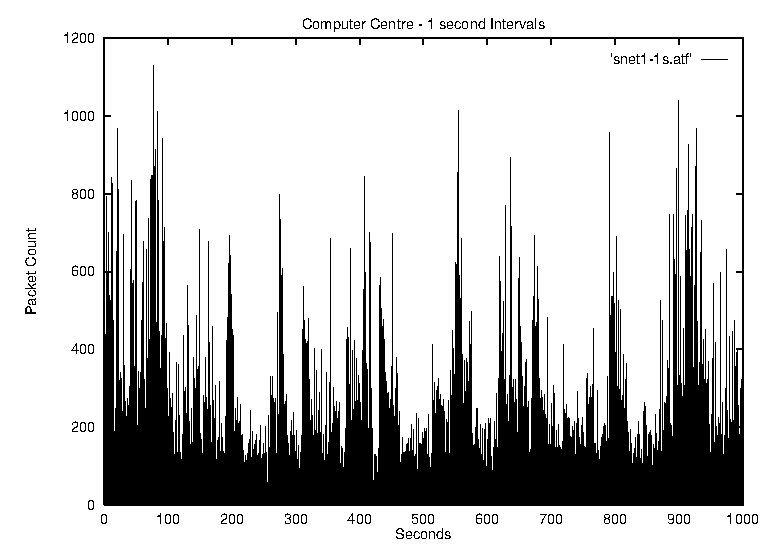
\includegraphics[height=3in]{pics/snet1-1s-freq.eps}
\caption{Computer Centre network with time interval 1 second}
\label{results:snet1.1s.freq}
\end{figure}

\begin{figure}
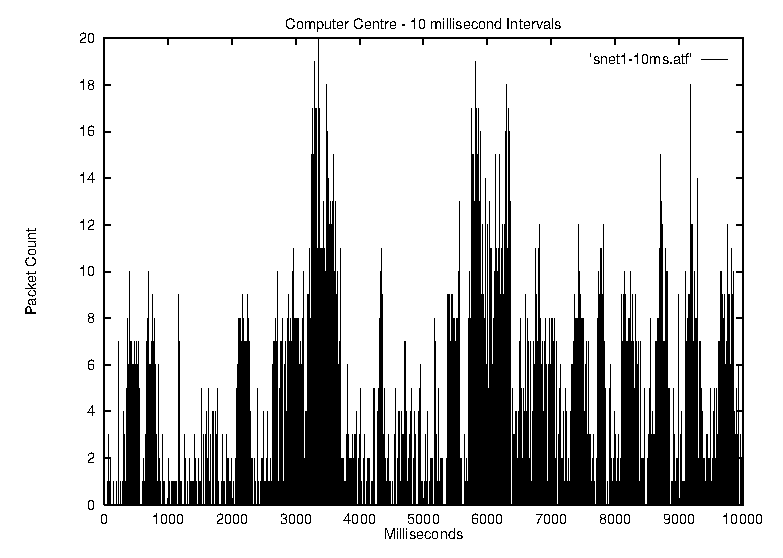
\includegraphics[height=3in]{pics/snet1-10ms-freq.eps}
\caption{Computer Centre network with time interval 10 milliseconds}
\label{results:snet1.10ms.freq}
\end{figure}

\begin{figure}
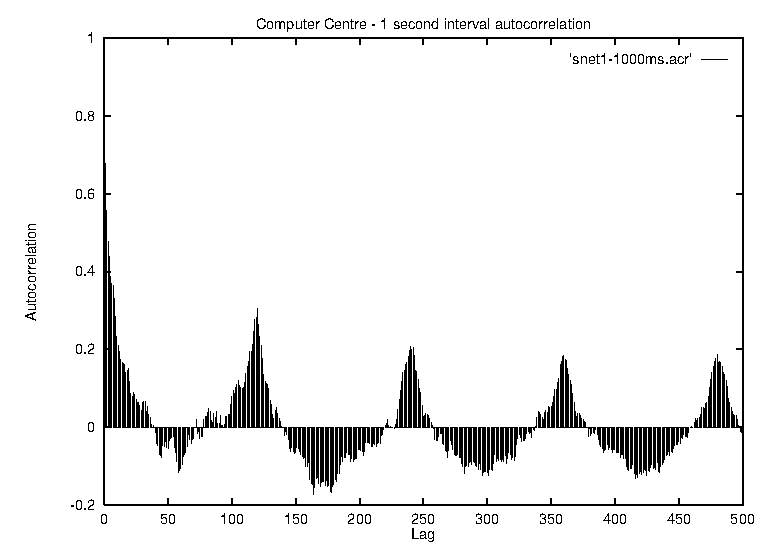
\includegraphics[height=3in]{pics/snet1-1s-acr.eps}
\caption{Computer Centre network autocorrelation with time interval 1 second}
\label{results:snet1.1s.acr}
\end{figure}

\begin{figure}
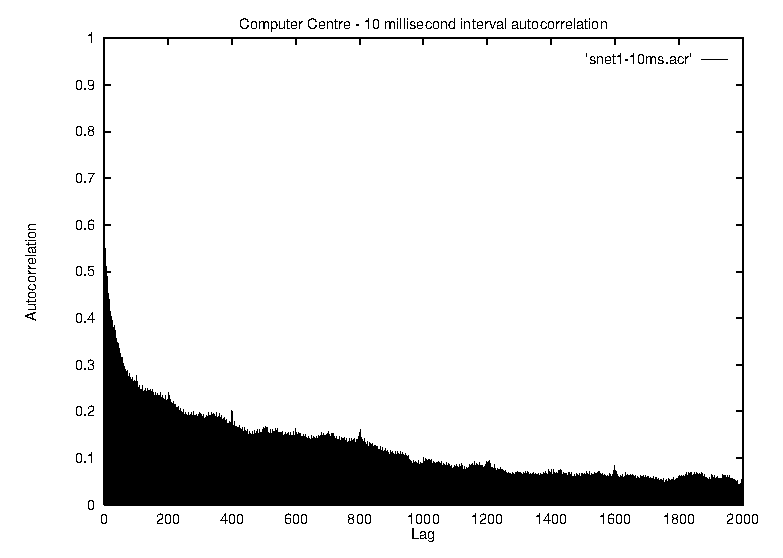
\includegraphics[height=3in]{pics/snet1-10ms-acr.eps}
\caption{Computer Centre network autocorrelation with time interval 10 milliseconds}
\label{results:snet1.10ms.acr}
\end{figure}

\begin{figure}
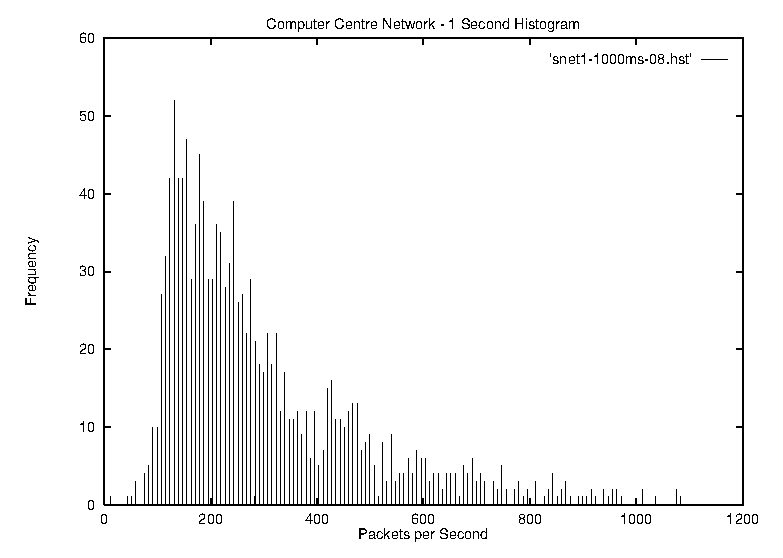
\includegraphics[height=3in]{pics/snet1-1s-hist-08.eps}
\caption{Computer Centre network histogram with time interval 1 second}
\label{results:snet1.1s.hist}
\end{figure}

Figure~\ref{results:snet1.1s.freq} shows the 1,000 seconds of sample
taken from subnet 1 of the Computer Centre staff network.  This
traffic has a steady background level of traffic with frequent bursts.
In figure~\ref{results:snet1.1s.acr} a definite 120 second cycle can
be observed.  This is caused by the router sending out NetWare Service
Broadcasts.  The router collects information about every NetWare file
server and print spooler and redistributes this information every two
minutes.  This amounts to about 500 Kbytes of information which is
sent using back to back maximum sized packets.
Figure~\ref{results:snet1.10ms.acr} shows the autocorrelation of the
10 millisecond interval results.  In this autocorrelation there exists
an underlying positive dependency.

The histogram (figure \ref{results:snet1.1s.hist}) shows a wide range
of traffic flow and that along with steady (and not insignificant)
background traffic, the bursts are both large in number and size.

\subsubsection{Department of Statistics network}

\begin{figure}
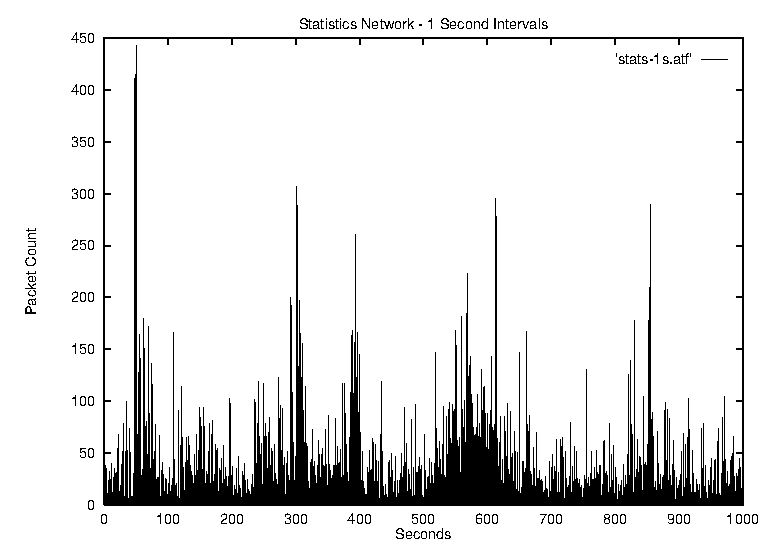
\includegraphics[height=3in]{pics/snet93-1s-freq.eps}
\caption{Statistics network with time interval 1 second}
\label{results:snet93.1s.freq}
\end{figure}

\begin{figure}
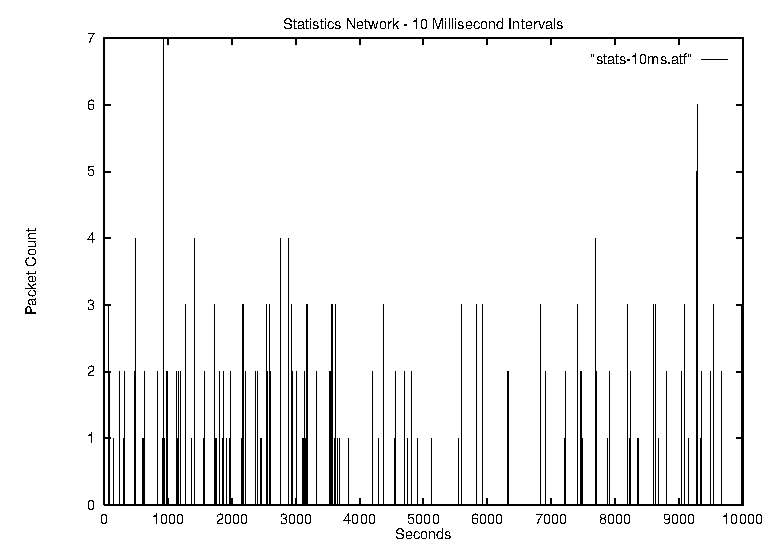
\includegraphics[height=3in]{pics/snet93-10ms-freq.eps}
\caption{Statistics network with time interval 10 milliseconds}
\label{results:snet93.10ms.freq}
\end{figure}

\begin{figure}
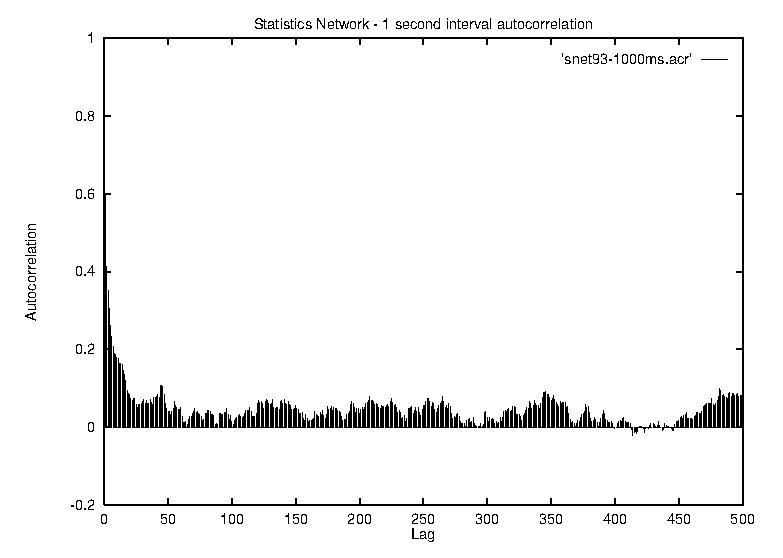
\includegraphics[height=3in]{pics/snet93-1s-acr.eps}
\caption{Statistics network autocorrelation with time interval 1 second}
\label{results:snet93.1s.acr}
\end{figure}

\begin{figure}
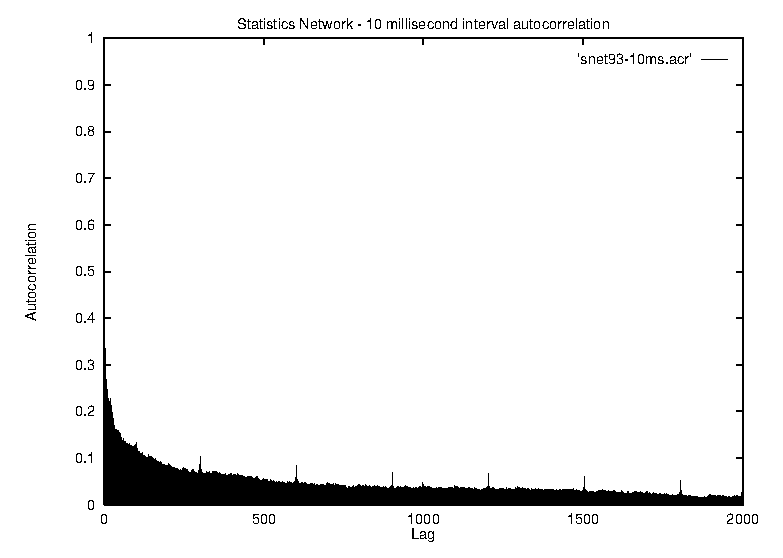
\includegraphics[height=3in]{pics/snet93-10ms-acr.eps}
\caption{Statistics network autocorrelation with time interval 10 milliseconds}
\label{results:snet93.10ms.acr}
\end{figure}

\begin{figure}
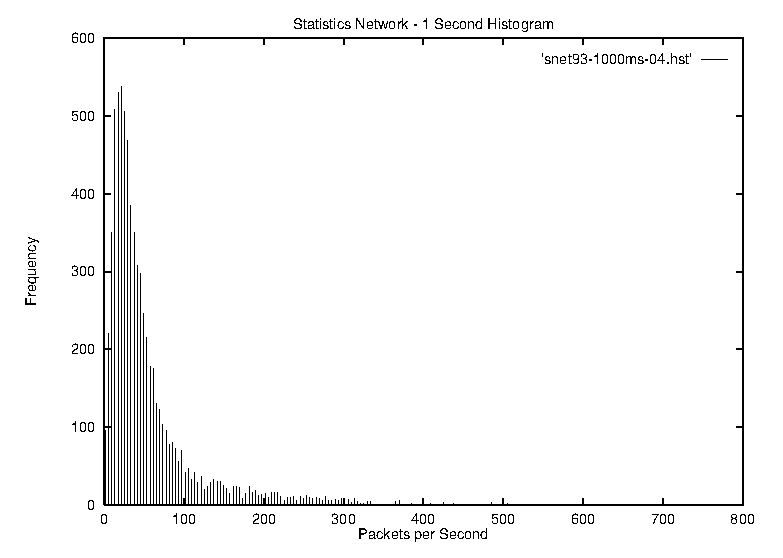
\includegraphics[height=3in]{pics/snet93-1s-hist-04.eps}
\caption{Statistics network histogram with time interval 1 second}
\label{results:snet93.1s.hist}
\end{figure}

The Department of Statistics staff subnetwork (also known as subnet
93) consists of about twenty Sun workstations using NIS and NFS
and some Macintoshes.  Apart from file and print server traffic it
also carries some X-windows traffic.

Figure~\ref{results:snet93.1s.freq} shows a much more lightly loaded
segment with minimal background traffic but still exhibiting very
bursty traffic.  The 10 millisecond autocorrelation
(figure~\ref{results:snet93.10ms.acr}) shows definite peaks every 300
milliseconds.  This is caused by the router broadcasting IP routeing
information.  It is not a very large amount of information (about
seven small sized packets sent back to back) indicating that the level
of background traffic is small (since it does not mask the route
broadcasts).  The histogram (figure ~\ref{results:snet93.1s.hist})
shows most of the traffic flows at a steady level and that bursts are
low in number and size.

\subsubsection{External gateway network of the University}

\begin{figure}
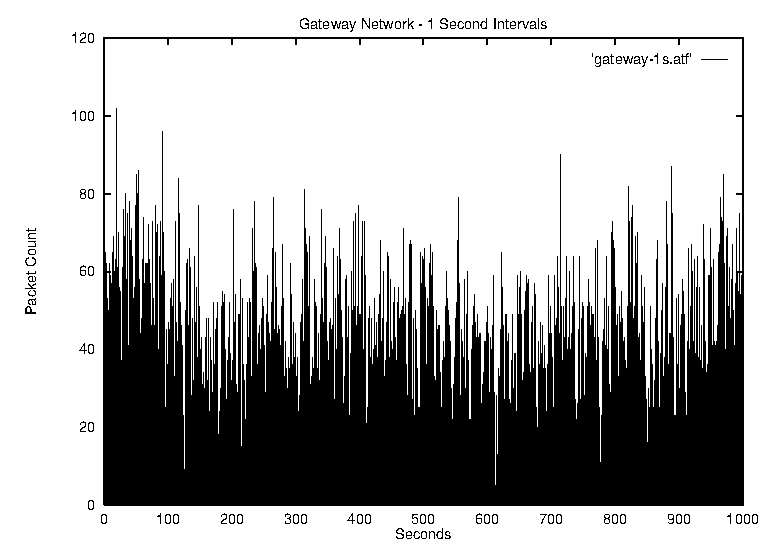
\includegraphics[height=3in]{pics/gatew-1s-freq.eps}
\caption{Gateway network with time interval 1 second}
\label{results:gatew.1s.freq}
\end{figure}

\begin{figure}
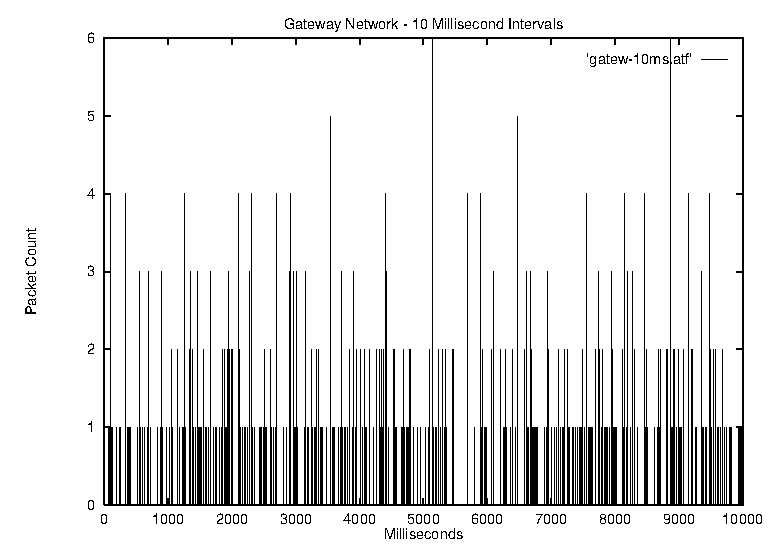
\includegraphics[height=3in]{pics/gatew-10ms-freq.eps}
\caption{Gateway network with time interval 10 millisecond}
\label{results:gatew.10ms.freq}
\end{figure}

\begin{figure}
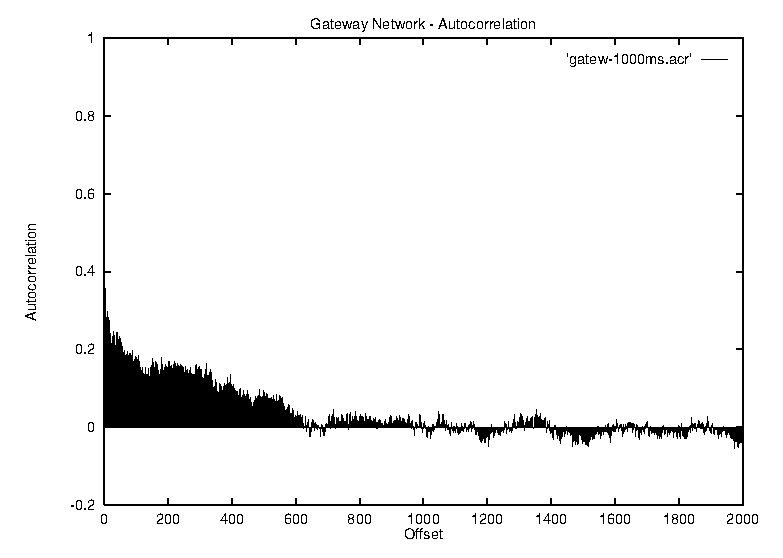
\includegraphics[height=3in]{pics/gatew-1s-acr.eps}
\caption{Gateway network autocorrelation with time interval 1 second}
\label{results:gatew.1s.acr}
\end{figure}

\begin{figure}
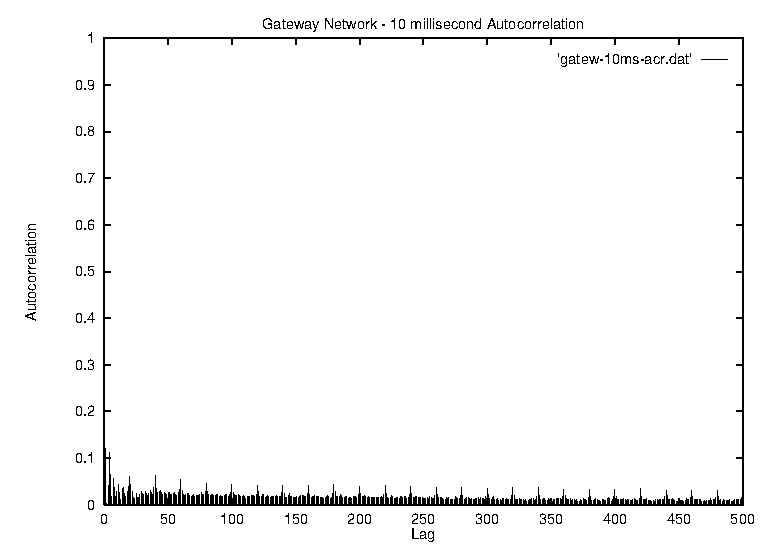
\includegraphics[height=3in]{pics/gatew-10ms-acr.eps}
\caption{Gateway network autocorrelation with time interval 10 milliseconds}
\label{results:gatew.10ms.acr}
\end{figure}

\begin{figure}
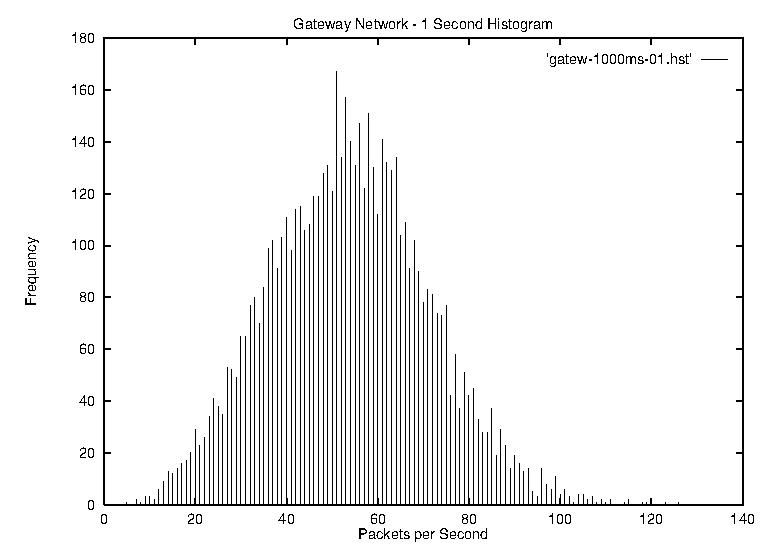
\includegraphics[height=3in]{pics/gatew-1s-hist-01.eps}
\caption{Gateway network histogram with time interval 1 second}
\label{results:gatew.1s.hist}
\end{figure}

The Gateway Network (figure~\ref{results:gatew.1s.freq}) has an
extremely light load with a considerable amount (with respect to the
total) of the traffic as a steady background flow.  The bursts are
much smaller in comparison to the other segments, with virtually all
the traffic consisting of TCP/IP.  The 1 second autocorrelation
(figure
\ref{results:gatew.1s.acr}) shows that there exists a dependency that
decays steadily with lag until it becomes noise around the 10 minute
lag time.  The 10 millisecond autocorrelation (figure
\ref{results:gatew.10ms.acr}) shows periodic behaviour every 200
milliseconds.  I am uncertain as to its exact cause but it could well
be Network Time Protocol (NTP) \cite{RFC:1305}.

The histogram (figure \ref{results:gatew.1s.hist}) shows very steady
traffic flows without any large bursts.  This link is connected to a
128 kbit connection to the outside world so the size of bursts would
be limited in any case but the unimodal, approximately symmetric shape
of the histogram most likely comes from the steady flow of USENET
traffic and the congestion control used by TCP.

\subsubsection{Commerce postgraduate teaching laboratory}

\begin{figure}
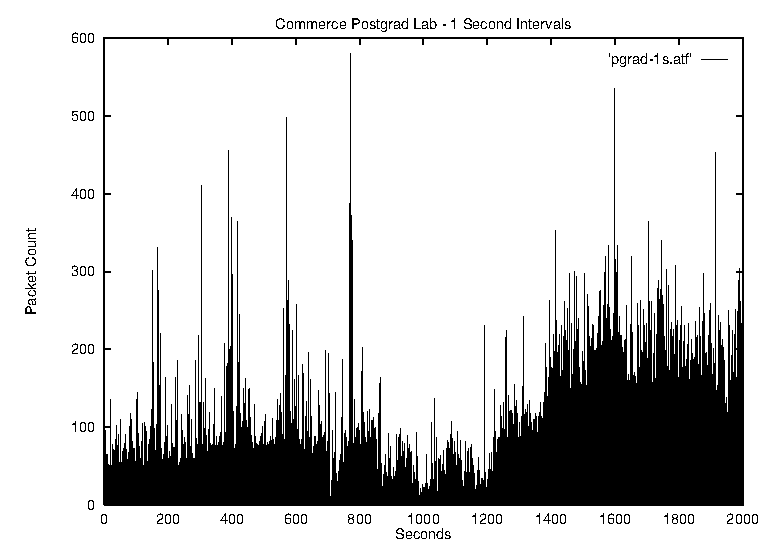
\includegraphics[height=3in]{pics/pgrad-1s-freq.eps}
\caption{Commerce Postgraduate Lab with time interval 1 second}
\label{results:pgrad.1s.freq}
\end{figure}


\begin{figure}
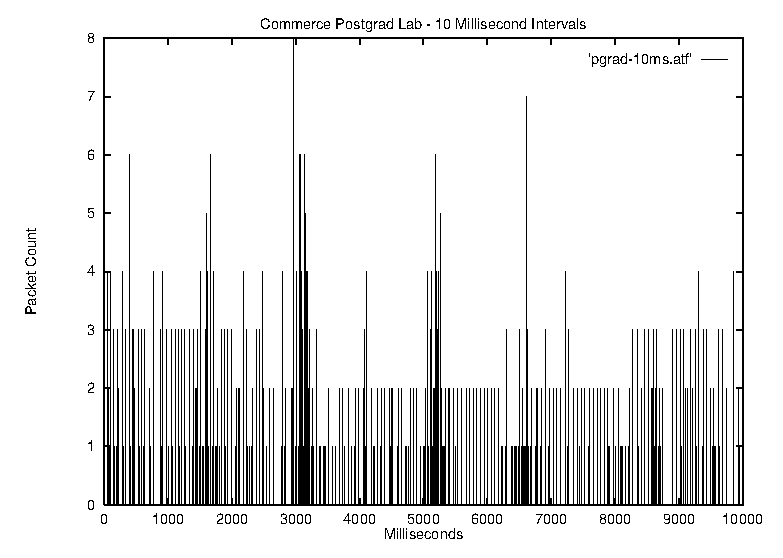
\includegraphics[height=3in]{pics/pgrad-10ms-freq.eps}
\caption{Commerce Postgraduate Lab with time interval 10 milliseconds}
\label{results:pgrad.10ms.freq}
\end{figure}

\begin{figure}
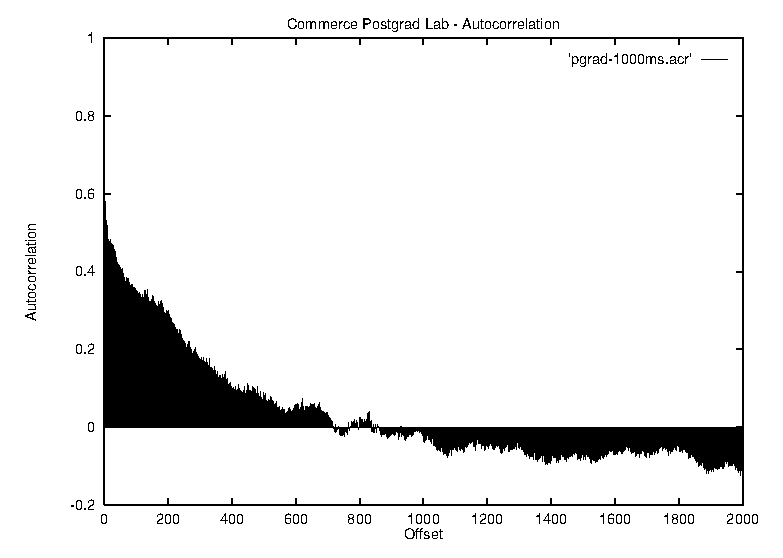
\includegraphics[height=3in]{pics/pgrad-1s-acr.eps}
\caption{Commerce Postgraduate Lab autocorrelation with time interval 1 second}
\label{results:pgrad.1s.acr}
\end{figure}

\begin{figure}
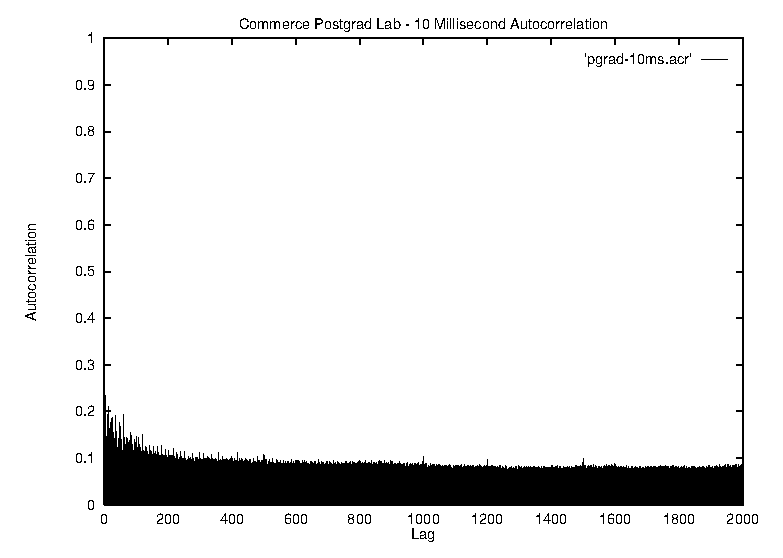
\includegraphics[height=3in]{pics/pgrad-10ms-acr.eps}
\caption{Commerce Postgraduate Lab autocorrelation with time interval 10 milliseconds}
\label{results:pgrad.10ms.acr}
\end{figure}

\begin{figure}
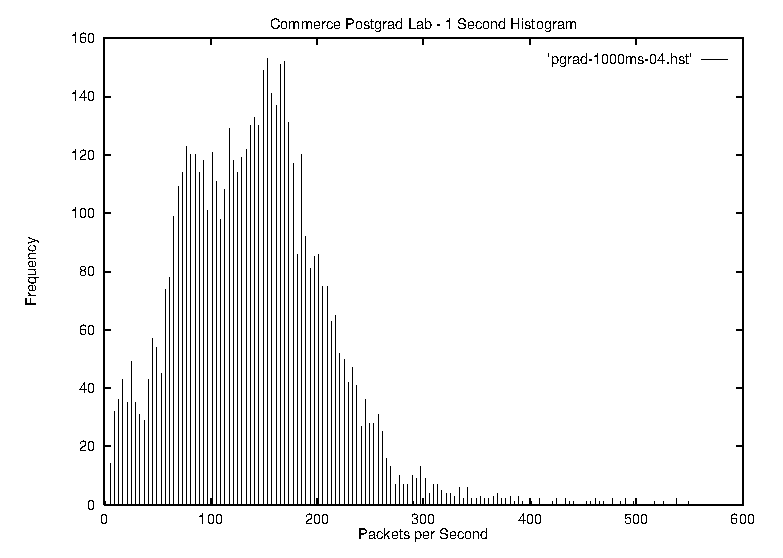
\includegraphics[height=3in]{pics/pgrad-1s-hist-04.eps}
\caption{Commerce Postgraduate histogram Lab with time interval 1 second}
\label{results:pgrad.1s.hist}
\end{figure}

The Commerce Postgraduate teaching laboratory consists of about twenty
personal computers running Windows For Workgroups.  They connect to a
Windows NT server using the NetBIOS LAN protocol.

This segment has a reasonably heavy load and only has NetBIOS traffic.
The down loading of large windows applications (over two megabytes or
more) creates large bursts of traffic.

NetBIOS has no routeing information and no directory system so there
is minimal periodic background traffic.  The figures
\ref{results:pgrad.1s.freq} and \ref{results:pgrad.10ms.freq} show a
steady level of traffic with only a few notable peaks.  This behaviour
is echoed in the histogram (figure \ref{results:pgrad.1s.hist})
showing that most of the traffic occured as steady flows.

\subsection{Graphs by protocol}

Below are three graphs showing the most prevalent protocols used
around the university, that is IP (\S \ref{network:ip}, AppleTalk (\S 
\ref{network:appletalk}) and Netware IPX (\S \ref{network:ipx}).

\subsubsection{Internet Protocol}

\begin{figure}
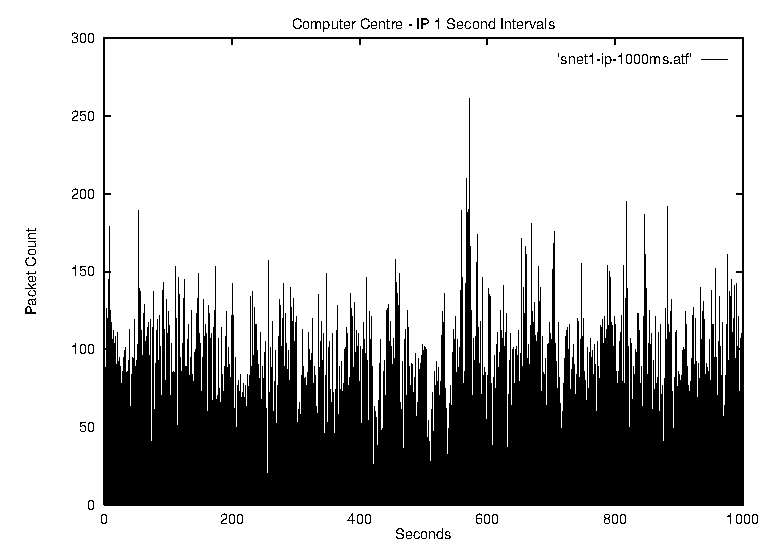
\includegraphics[height=3in]{pics/snet1-ip-1s-freq.eps}
\caption{IP traffic on Computer Centre network with time interval 1 second}
\label{results:snet1.ip.1s.freq}
\end{figure}

\begin{figure}
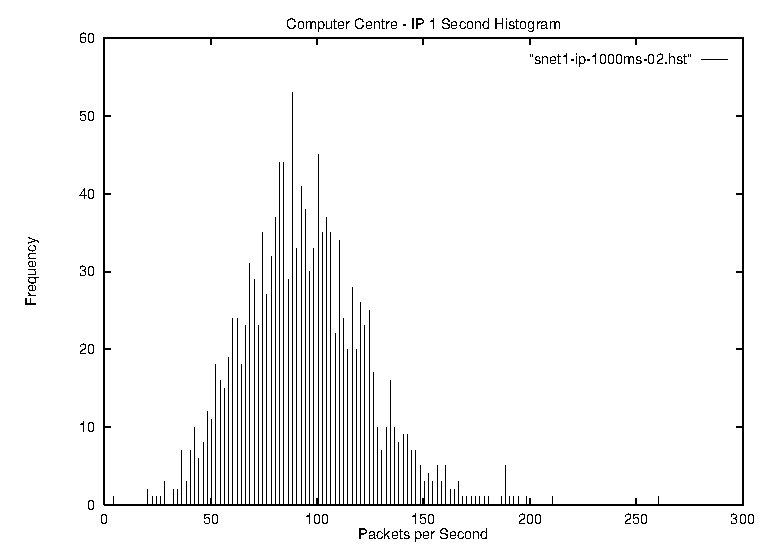
\includegraphics[height=3in]{pics/snet1-ip-1s-hist-02.eps}
\caption{Histogram of IP traffic on Computer Centre network with time interval 1 second}
\label{results:snet1.ip.1s.hist}
\end{figure}


Figure~\ref{results:snet1.ip.1s.freq} shows Internet Protocols traffic.
This graph shows a reasonable (with respect to the peak maximums)
amount of background traffic.  This is most likely a result of a
steady level of remote login and mail traffic.

\subsubsection{AppleTalk}

\begin{figure}
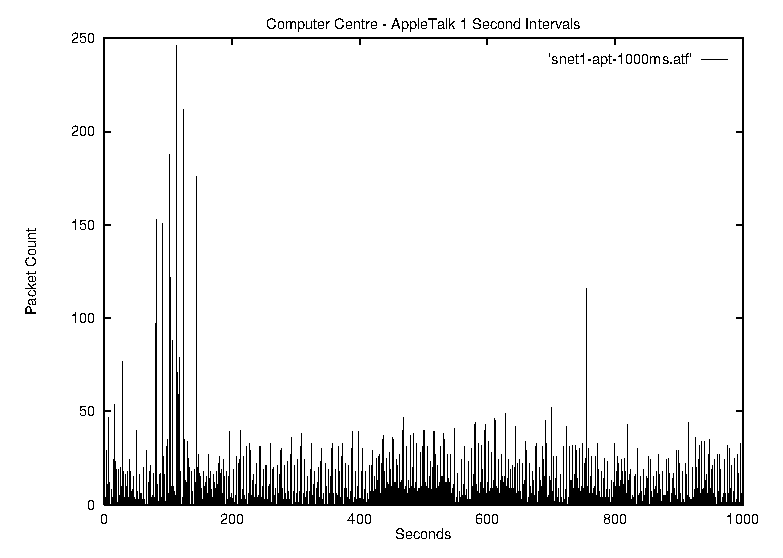
\includegraphics[height=3in]{pics/snet1-apt-1s-freq.eps}
\caption{AppleTalk traffic on Computer Centre network with time interval 1 second}
\label{results:snet1.apt.1s.freq}
\end{figure}

\begin{figure}
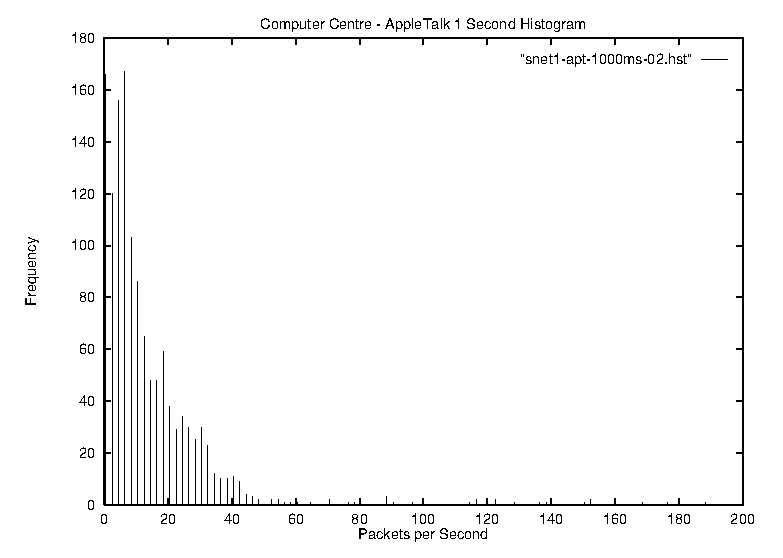
\includegraphics[height=3in]{pics/snet1-apt-1s-hist-02.eps}
\caption{Histogram of AppleTalk traffic on Computer Centre network with time interval 1 second}
\label{results:snet1.apt.1s.hist}
\end{figure}

Figure~\ref{results:snet1.apt.1s.freq} shows AppleTalk traffic on the
Computer Centre network.  Because there is very little AppleTalk
traffic on subnet 1 events become more pronounced and noticeable.
AppleTalk has periodic broadcasts to relay routeing and directory
services (zone maps) information.

\subsubsection{Netware IPX}

\begin{figure}
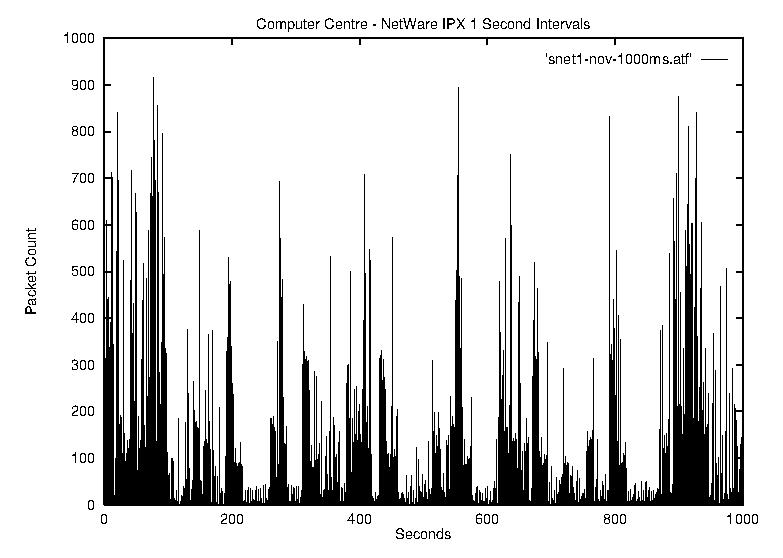
\includegraphics[height=3in]{pics/snet1-ipx-1s-freq.eps}
\caption{IPX traffic on Computer Centre network with time interval 1 second}
\label{results:snet1.nov.1s.freq}
\end{figure}

\begin{figure}
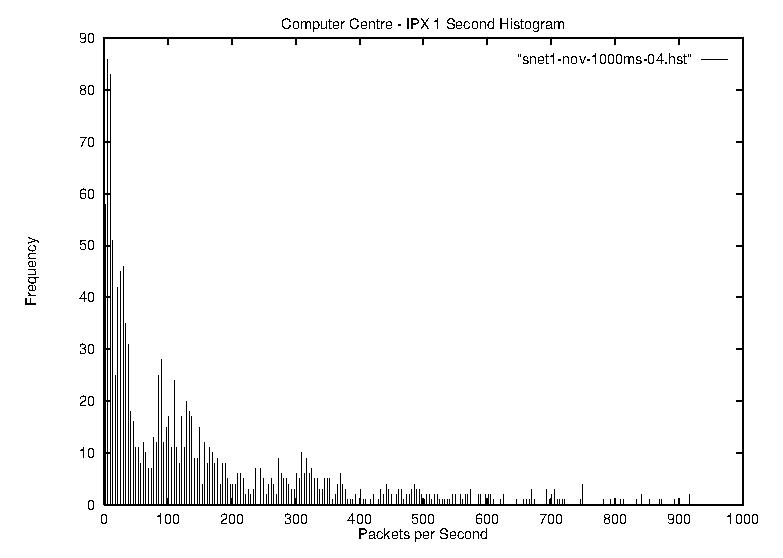
\includegraphics[height=3in]{pics/snet1-ipx-1s-hist-02.eps}
\caption{Histogram of IPX traffic on Computer Centre network with time interval 1 second}
\label{results:snet1.nov.1s.hist}
\end{figure}

\begin{figure}
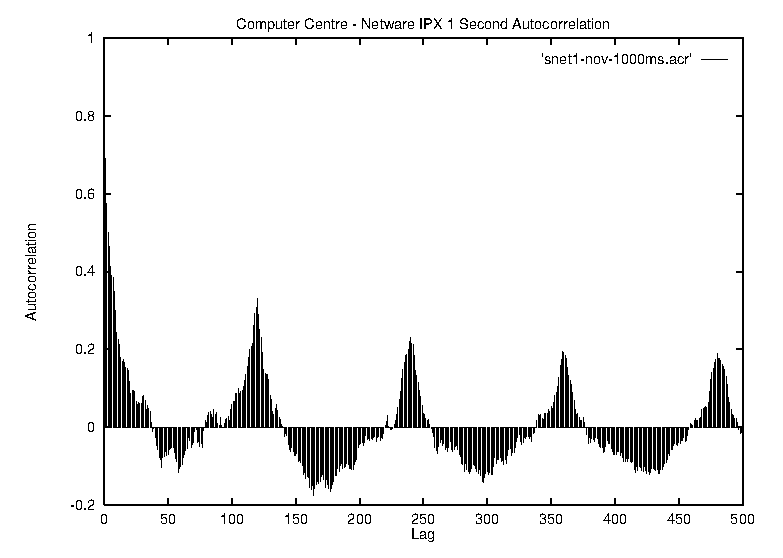
\includegraphics[height=3in]{pics/snet1-ipx-1s-acr.eps}
\caption{Autocorrelation of IPX traffic on Computer Centre network with time interval 1 second}
\label{results:snet1.nov.1s.acr}
\end{figure}

Figure~\ref{results:snet1.nov.1s.freq} show Netware traffic on the
Computer Centre network.  While it looks as though there is
considerable IPX traffic in fact there is little file transfer
traffic.  The large bursts of traffic come from Netware's service
announcements.  Every two minutes Netware capable routers broadcast
all available Netware services, such as file servers, printing
spoolers and mail exchanges.  Due to the number of these services
around the university it amounts to over 500 kilobytes of information.
This is clearly seen in the autocorrelation (figure
\ref{results:snet1.nov.1s.acr}).

\clearpage

\section{Slowly decaying variance}

Figures \ref{results:snet1.10ms.sta}, \ref{results:gatew.10ms.sta},
\ref{results:snet93.10ms.sta} and \ref{results:pgrad.10ms.sta} all
show the slowly decaying variance associated with self-similar
behaviour.  The plots are created from the output of \texttt{stat}
program (\S \ref{results:stat}.  The plots use the logarithm base 10
output from \texttt{stat}.  This is the same as the slowly decaying
variance plots in the Bellcore papers \cite{Bell:1} \cite{Bell:2}.
Each plot includes a line with slope $y = -x$ for reference (the
theoretical slope for a general renewal is $y = x^{-1}$, so taking the
logarithm gives $y = -x$).  While each plot is unique they all have a
similar shape and clearly show slowly decaying behaviour.

While is obvious that the shapes are different, because of the
differences in the samples there is no simple explanation as to how the
shape of the curve relates to the underlying traffic behaviour.

\begin{figure}
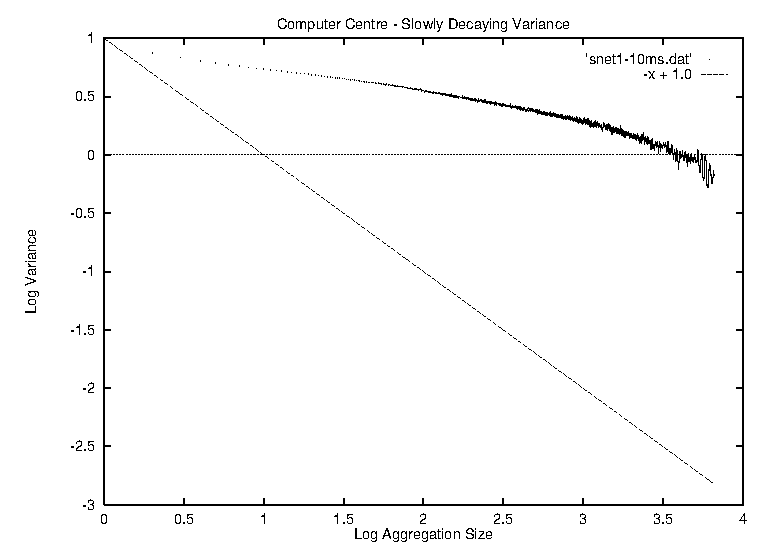
\includegraphics[height=3in]{pics/snet1-10ms-sta.eps}
\caption{Slowly decaying variance plot of the Computer Centre network}
\label{results:snet1.10ms.sta}
\end{figure}

\begin{figure}
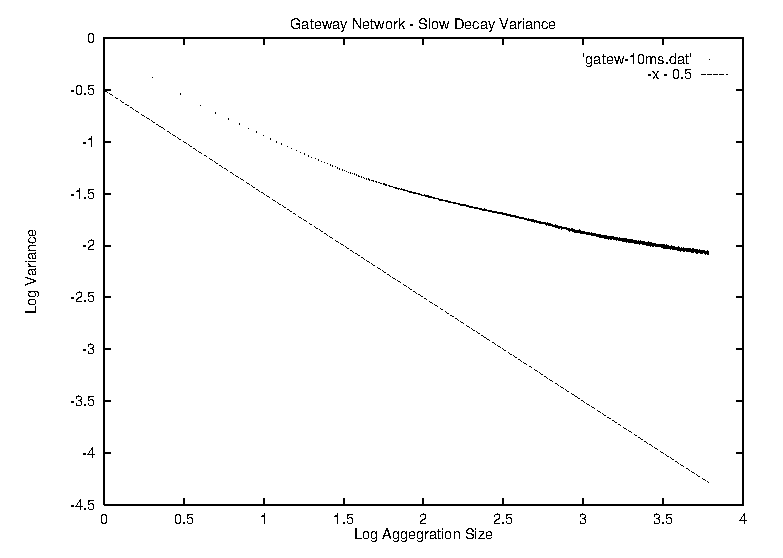
\includegraphics[height=3in]{pics/gatew-10ms-sta.eps}
\caption{Slowly decaying variance plot of the Gateway network}
\label{results:gatew.10ms.sta}
\end{figure}

\begin{figure}
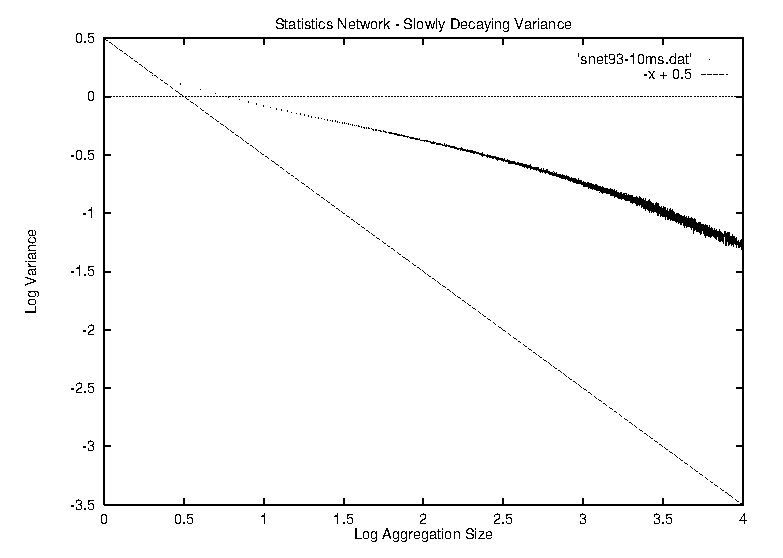
\includegraphics[height=3in]{pics/snet93-10ms-sta.eps}
\caption{Slowly decaying variance plot of the Statistics network}
\label{results:snet93.10ms.sta}
\end{figure}

\begin{figure}
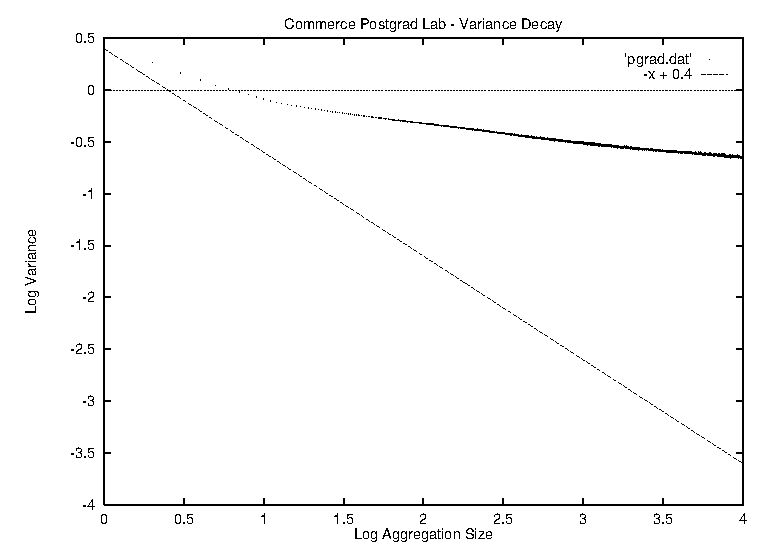
\includegraphics[height=3in]{pics/pgrad-10ms-sta.eps}
\caption{Slowly decaying variance plot of the Commerce Postgraduate network}
\label{results:pgrad.10ms.sta}
\end{figure}


\chapter{Simulation}
\label{simulation}

\section{Introduction}

A series of simulation experiments was performed.  Below is the list
of nine experiments.  Each experiment generated a sample trace of
length 1,000 seconds.

\begin{enumerate}
\item	Poisson process simulation.
\item	Renewal process with scaled uniform inter-renewal distribution.
\item	A 3-state modulated renewal process.
\item	Renewal process with Pareto (infinite variance) inter-renewal distribution.
\item	Renewal process with $t_2-distribution$ (infinite variance) inter-renewal distribution.
\item	Renewal process with Cauchy inter-renewal (infinite variance) distribution.
\item	Single renewal process with $t_2-distribution$ inter-renewal distribution.
\item	10 super-imposed independent renewal processes with $t_2-distribution$ inter-renewal distributions.
\item	100 super-imposed independent renewal processes with $t_2-distribution$ inter-renewal distributions.
\end{enumerate}

The simulations were done using a single chain of recurrent events,
ordered by time.  Each event is independent of all others on the
chain, and knows when in the future it will occur.  The chain also has
a notion of the current time.  When an event reaches the head of the
chain it occurs and is recorded into the trace file.  The current time
is set to the time of the event and a new time for it to occur is
generated.  This event (now to occur sometime in the future) is placed
back into the chain in chronological order.

The events are self contained and may have simple (samples from some
distribution) or complex (with multiple internal states) recurrent
behaviour.  All that is required is that it generates a new recurrence
time in the positive future.

\section{Simulation of simple Poisson process}
\label{simulation:simplepp}

Using the simplest model available, that is exponentially distributed
inter-arrival times, we can produce sample traces to examine.  This
simulation is not meant to be comparable to the real traces, but
rather a counter example to show that such a model does not fit
Ethernet traffic patterns.

It is also intended to show that the simulation techniques work
properly and that the tools developed to produce the results are
robust.

\subsection{Exponential arrival distribution}

\begin{figure}
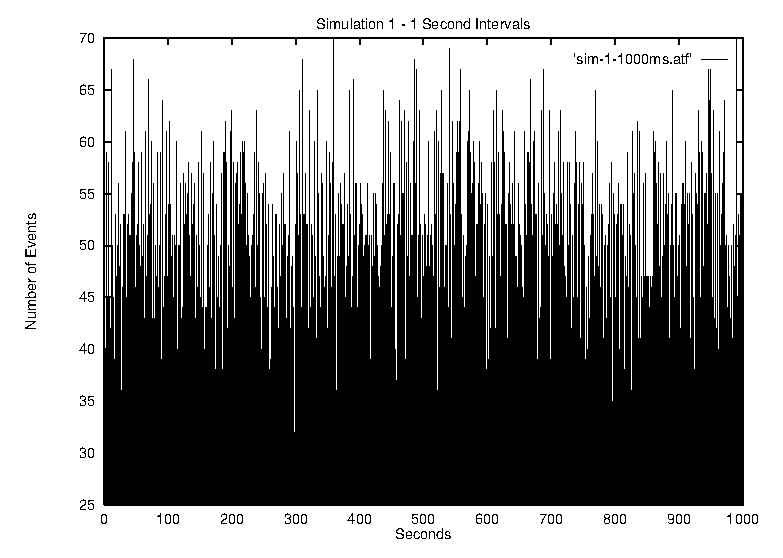
\includegraphics[height=3in]{pics/sim-1-1s-freq.eps}
\caption{Poisson Process Simulation with Exponential Distribution}
\label{simulation:sim1.1s.freq}
\end{figure}

\begin{figure}
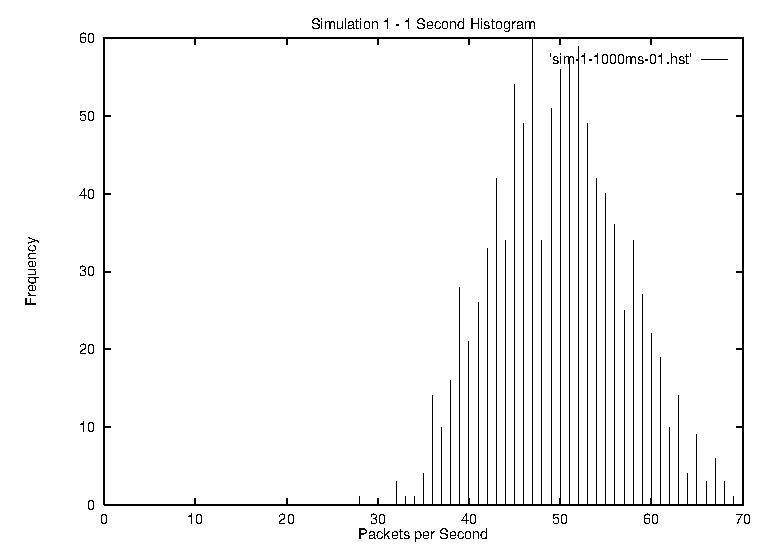
\includegraphics[height=3in]{pics/sim-1-1s-hist-01.eps}
\caption{Histogram of a Poisson Process Simulation}
\label{simulation:sim1.1s.hist}
\end{figure}

\begin{figure}
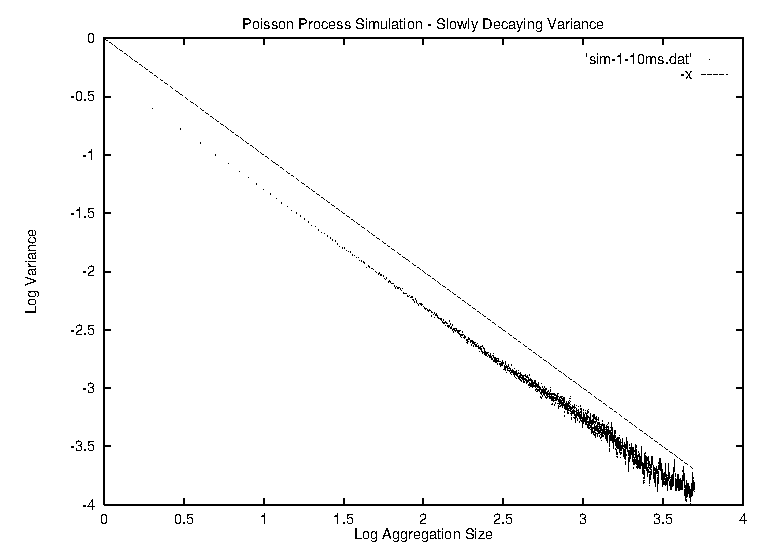
\includegraphics[height=3in]{pics/sim-1-10ms-sta.eps}
\caption{Slowly decaying variance plot of a Poisson Process Simulation}
\label{simulation:sim1.10ms.sta}
\end{figure}

The first simulation {\em sim-1} is a Poisson Process with rate
$\lambda = 0.05$ packets per millisecond, simulated over a period of
1,000 seconds ($\sim$ 16 minutes).  This results in an exponentially
distributed inter-arrival time with mean $\mu = 20$.  A sample trace
can be seen in figure~\ref{simulation:sim1.1s.freq} along with the
packet frequency histogram (figure~\ref{simulation:sim1.1s.hist}) and
slowly decaying variance plot
(figure~\ref{simulation:sim1.10ms.sta}).  As expected the plot is a
straight line with a slope of $-1$, hence the variance decays order
$n^{-1}$ with averaging aggregation, in line with the theoretical
model.

\subsection{Single state with uniform inter-arrival time distribution}

\begin{figure}
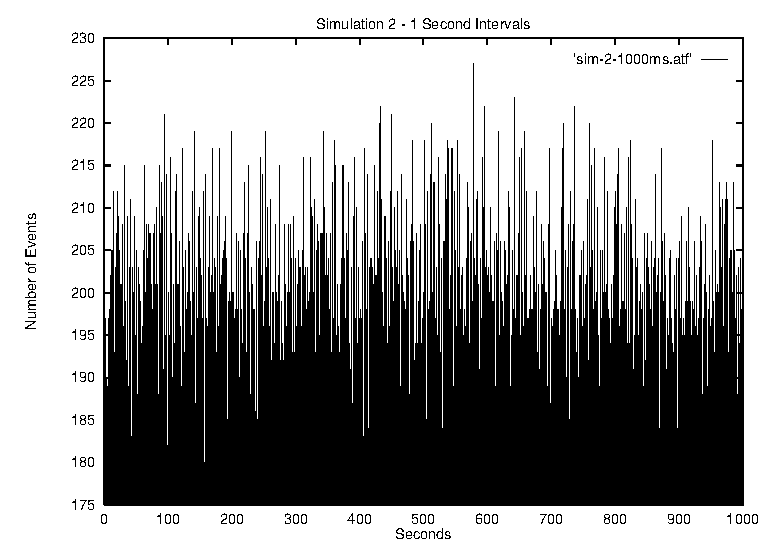
\includegraphics[height=3in]{pics/sim-2-1s-freq.eps}
\caption{Uniform Distribution Renewal Process Simulation}
\label{simulation:sim2.1s.freq}
\end{figure}

\begin{figure}
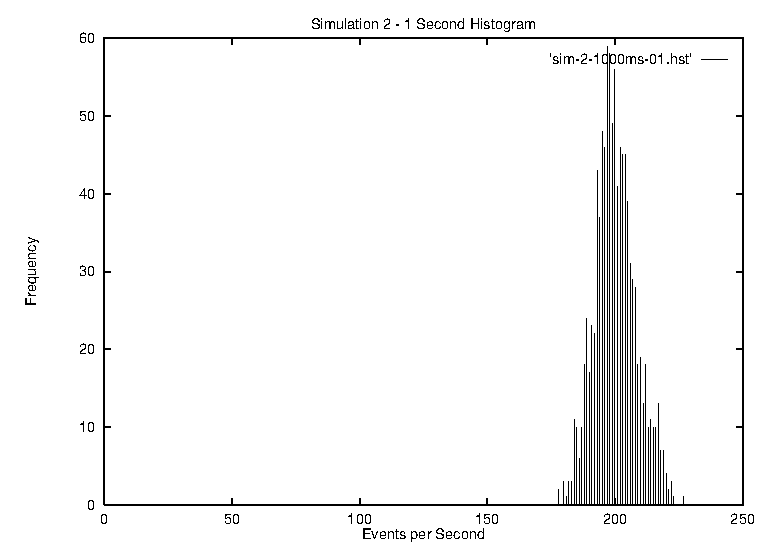
\includegraphics[height=3in]{pics/sim-2-1s-hist-01.eps}
\caption{Histogram of Uniform Distribution Renewal Process Simulation}
\label{simulation:sim2.1s.hist}
\end{figure}

\begin{figure}
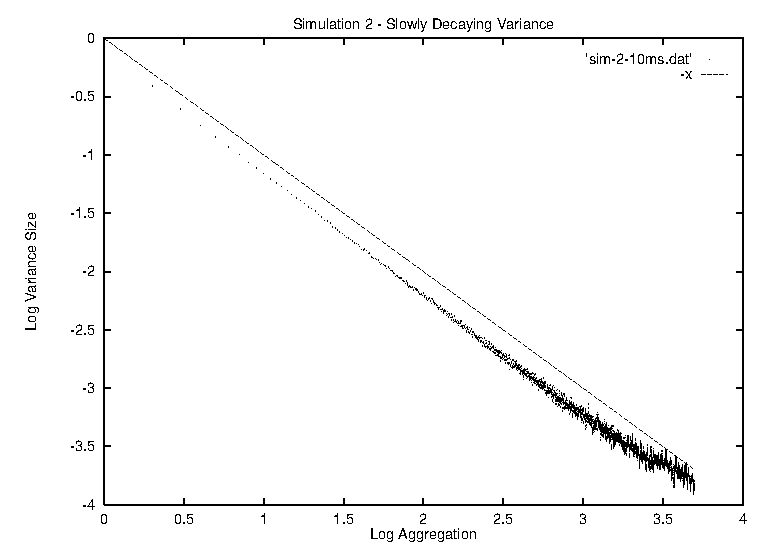
\includegraphics[height=3in]{pics/sim-2-10ms-sta.eps}
\caption{Slowly decaying variance plot of Uniform Distribution Renewal Process Simulation}
\label{simulation:sim2.10ms.sta}
\end{figure}

The second simulation \emph{sim-2} is a renewal process which has
inter-arrival times that are uniformly distributed with mean $\mu =
20$.  The time series can be seen in
figure~\ref{simulation:sim2.1s.freq} along with its histogram
(figure~\ref{simulation:sim2.1s.hist}) and the slowly decaying
variance plot (figure~\ref{simulation:sim2.10ms.sta}).  Again the
variance plot is a straight line with slope $-1$, that is it shows no
sign of self-similar behaviour.

\section{Generalised modulated renewal process}

\subsection{The model}

The mathematical model for this simulation is discussed in the models
chapter (\S \ref{models:genmodproc}).

\subsection{The program}

The program reads in a parameter file and produces a trace file
(Figure~\ref{trace:format}).

{\ttfamily \begin{flushleft}
  simulate [-t time in seconds] parameter files
\end{flushleft}}

\subsubsection{An example}

For an example I have chosen a three state process.

\bigskip

\begin{tabular}{||l||l|l||l|l||} \hline
State & \multicolumn{2}{l||}{Inter-Event Distribution} &
\multicolumn{2}{l||}{Lifetime Distribution} \\ \hline
 & Distribution & Mean & Distribution & Mean \\ \hline \hline
0 & Exponential & 10 & Exponential & 100 \\ \hline
1 & Deterministic & 2 & Uniform & 40 \\ \hline
2 & Deterministic & 1 & Deterministic & 15 \\ \hline
\end{tabular}

\bigskip

\begin{figure}
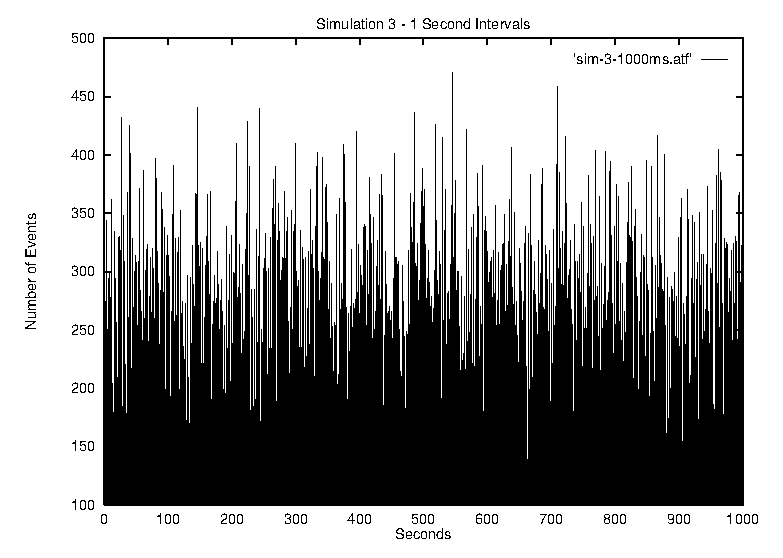
\includegraphics[height=3in]{pics/sim-3-1s-freq.eps}
\caption{Modulated Renewal Process Simulation}
\label{simulation:sim3.1s.freq}
\end{figure}

\begin{figure}
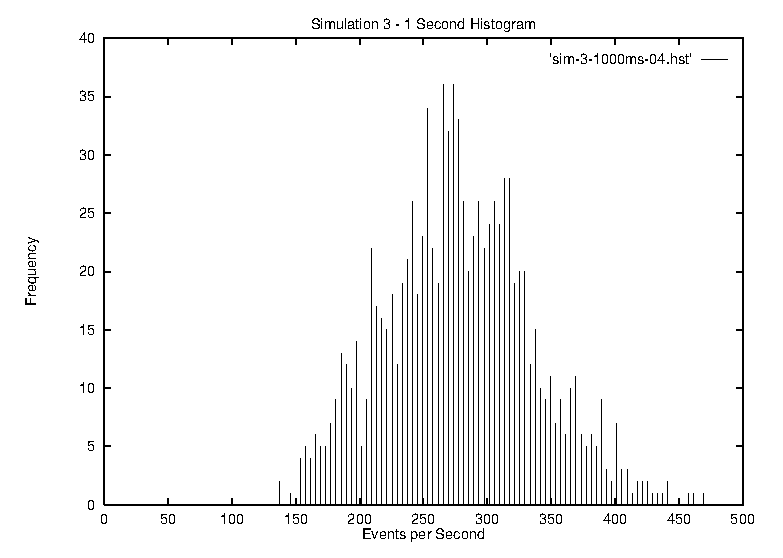
\includegraphics[height=3in]{pics/sim-3-1s-hist-04.eps}
\caption{Histogram of Modulated Renewal Process Simulation}
\label{simulation:sim3.1s.hist}
\end{figure}

\begin{figure}
\includegraphics[height=3in]{pics/sim-3-10ms-acr.eps}
\caption{Autocorrelation of Modulated Renewal Process Simulation}
\label{simulation:sim3.10ms.acr}
\end{figure}

\begin{figure}
\includegraphics[height=3in]{pics/sim-3-10ms-sta.eps}
\caption{Slowly decaying variance plot of Modulated Renewal Process Simulation}
\label{simulation:sim3.10ms.sta}
\end{figure}

The results of the simulation \emph{sim-3} are shown in figures
\ref{simulation:sim3.1s.freq}, \ref{simulation:sim3.1s.hist},
\ref{simulation:sim3.10ms.acr} and \ref{simulation:sim3.10ms.sta}.
The time series (figure \ref{simulation:sim3.1s.freq}) looks bursty
but the histogram (figure \ref{simulation:sim3.1s.hist} shows that the
number of large bursts is small and that most of the flows are in a
limited range (200 -- 350 events per second).

The autocorrelation (figure \ref{simulation:sim3.10ms.acr}) shows the
existence of a definite short term correlation, caused by the
deterministic behaviour within two of the states.  This short term
correlation falls away in relation to the expected life time of the
deterministic states to white noise caused by the Poisson distributed
state and life time.

The slowly decaying variance graph (figure
\ref{simulation:sim3.10ms.sta}) shows that this model is not what we
are looking for, and that a more complex model does not help.

\clearpage

\section{Infinite variance renewal processes}

\subsection{Introduction}

Below are the results of three simple renewal processes, similar to
the simple Poisson process (\S \ref{simulation:simplepp}) except that
the inter-renewal distributions have infinite variance.  This class
(having infinite variance) of distributions is often known as
heavy-tailed distributions.

The three distributions used are the Pareto distribution, a non
symmetric distribution that is defined on ${\mathbb R}^+$.  This
distribution was used because of its reference in \cite{Bell:4} (\S
3.2.3, Page 19).  The Pareto distribution is a stable distribution
making further mathematical analysis a little simpler than other
distributions.

The other two distributions come from Student's $t$ distribution.  For
degrees of freedom 1 and 2 it has infinite variance.  The
$t_1-distribution$, commonly known as the Cauchy distribution, also
has infinite mean.  The $t_\nu-distribution$ is a flattened normal,
symmetric and defined on all of ${\mathbb R}$.  For the simulations
the distributions are folded around the y-axis so that only positive
inter-renewal times exist.

\subsection{Pareto distribution}

\begin{figure}
\includegraphics[height=3in]{pics/sim-4-1s-freq.eps}
\caption{Pareto Distributed Renewal Process Simulation}
\label{simulation:sim4.1s.freq}
\end{figure}

\begin{figure}
\includegraphics[height=3in]{pics/sim-4-1s-hist-01.eps}
\caption{Histogram of Pareto Distributed Renewal Process Simulation}
\label{simulation:sim4.1s.hist}
\end{figure}

\begin{figure}
\includegraphics[height=3in]{pics/sim-4-10ms-acr.eps}
\caption{Autocorrelation of Pareto Distributed Renewal Process Simulation}
\label{simulation:sim4.10ms.acr}
\end{figure}

\begin{figure}
\includegraphics[height=3in]{pics/sim-4-10ms-sta.eps}
\caption{Slowly decaying variance plot of Pareto Distributed Renewal Process Simulation}
\label{simulation:sim4.10ms.sta}
\end{figure}

The time series for \emph{sim-4} is shown in figure
\ref{simulation:sim4.1s.freq}.  The large number of gaps and lack of
``background'' traffic are notable features of this plot (the
$t-distribution$ plots also show this behaviour).  The histogram
(figure \ref{simulation:sim4.1s.hist}) shows a wide range of traffic
levels.  Note that although it cannot be seen there is bar of height
143 at 0 events per second.

The autocorrelation (figure \ref{simulation:sim4.10ms.acr}) displays
the important positive autocorrelation, indicating long range
dependence.  The slowly decaying variance (figure
\ref{simulation:sim4.10ms.sta}) shows the decay occuring at a slower
rate than $x^{-1}$, verifying that infinite variance renewal processes
do exhibit fractal behaviour.

\subsection{Cauchy and $t$ distributions}

\begin{figure}[h]
\includegraphics[height=3in]{pics/sim-5-1s-freq.eps}
\caption{$t_2-distribution$ Distributed Renewal Poisson Simulation}
\label{simulation:sim5.1s.freq}
\end{figure}

\begin{figure}
\includegraphics[height=3in]{pics/sim-5-10ms-acr.eps}
\caption{Autocorrelation of $t_2-distribution$ Distributed Renewal Process Simulation}
\label{simulation:sim5.10ms.acr}
\end{figure}

\begin{figure}
\includegraphics[height=3in]{pics/sim-5-10ms-sta.eps}
\caption{Slowly decaying variance plot of $t_2-distribution$ Distributed Renewal Process Simulation}
\label{simulation:sim5.10ms.sta}
\end{figure}


\begin{figure}
\includegraphics[height=3in]{pics/sim-6-1s-freq.eps}
\caption{Cauchy Distributed Renewal Poisson Simulation}
\label{simulation:sim6.1s.freq}
\end{figure}

\begin{figure}
\includegraphics[height=3in]{pics/sim-6-10ms-acr.eps}
\caption{Autocorrelation of Cauchy Distributed Renewal Process Simulation}
\label{simulation:sim6.10ms.acr}
\end{figure}

\begin{figure}
\includegraphics[height=3in]{pics/sim-6-10ms-sta.eps}
\caption{Slowly decaying variance plot of Cauchy Distributed Renewal Process Simulation}
\label{simulation:sim6.10ms.sta}
\end{figure}

Figures \ref{simulation:sim5.1s.freq}, \ref{simulation:sim5.10ms.acr}
and \ref{simulation:sim5.10ms.sta} are the result from simulating a
general renewal process with a $t_2-distribution$ inter-renewal
distribution (\emph{sim-5}).

Figures \ref{simulation:sim6.1s.freq}, \ref{simulation:sim6.10ms.acr}
and \ref{simulation:sim6.10ms.sta} are the result from simulating a
general renewal process with a Cauchy ($t_1-distribution$) inter-renewal
distribution (\emph{sim-6}).

The Cauchy distribution simulation generated very few (in comparison
with the other simulations and real samples) events so that the
analysis is less reliable.  The $t_2-distribution$ results show strong
positive autocorrelation and noticeable slowly decaying variance.

\clearpage

\subsection{Merged $t_2-distribution$ renewal processes}

Below are the results for the superimposed (or merged) renewal
processes.  The full definition can be found in the models chapter (\S
\ref{models:mergedprocs}).  The base distribution is a $t_2-distribution$.
This was used as it produced clear results in the earlier simulations.
The choice of the $t_2-distribution$ rather than Pareto was mainly one
of personal opinion and my impression that it gave a clearer results
with respect to slowly decaying variance and long range dependence
(the autocorrelation).  Earlier experiments show that the Pareto is a
perfectly acceptable distribution for these experiments and produces
similar conclusions.

A single process is repeated (identical in distribution to simulation
5) as a control (\emph{sim-7}). 10 and 100 merged processes were then
produced (\emph{sim-8} and \emph{sim-9} respectively).  Both of these
produced a large number of total events giving decisive results.

\begin{figure}[h]
\includegraphics[height=3in]{pics/sim-7-1s-freq.eps}
\caption{Single $t_2-distribution$ Distributed Renewal Process Simulation}
\label{simulation:sim7.1s.freq}
\end{figure}

\begin{figure}
\includegraphics[height=3in]{pics/sim-7-1s-hist-08.eps}
\caption{Histogram of Single $t_2-distribution$ Distributed Renewal Process Simulation}
\label{simulation:sim7.1s.hist}
\end{figure}

\begin{figure}
\includegraphics[height=3in]{pics/sim-7-10ms-acr.eps}
\caption{Autocorrelation of Single $t_2-distribution$ Distributed Renewal Process Simulation}
\label{simulation:sim7.10ms.acr}
\end{figure}

\begin{figure}
\includegraphics[height=3in]{pics/sim-7-10ms-sta.eps}
\caption{Slowly decaying variance plot of Single $t_2-distribution$ Distributed Renewal Process Simulation}
\label{simulation:sim7.10ms.sta}
\end{figure}

\begin{figure}
\includegraphics[height=3in]{pics/sim-8-1s-freq.eps}
\caption{10 Superimposed $t_2-distribution$ Distributed Renewal Process Simulation}
\label{simulation:sim8.1s.freq}
\end{figure}


\begin{figure}
\includegraphics[height=3in]{pics/sim-8-1s-hist-16.eps}
\caption{Histogram of 10 Superimposed $t_2-distribution$ Distributed Renewal Process Simulation}
\label{simulation:sim8.1s.hist}
\end{figure}

\begin{figure}
\includegraphics[height=3in]{pics/sim-8-10ms-acr.eps}
\caption{Autocorrelation of 10 Superimposed $t_2-distribution$ Distributed Renewal Process Simulation}
\label{simulation:sim8.10ms.acr}
\end{figure}

\begin{figure}
\includegraphics[height=3in]{pics/sim-8-10ms-sta.eps}
\caption{Slowly decaying variance plot of 10 Superimposed $t_2-distribution$ Distributed Renewal Process Simulation}
\label{simulation:sim8.10ms.sta}
\end{figure}

\begin{figure}[h]
\includegraphics[height=3in]{pics/sim-9-1s-freq.eps}
\caption{100 Superimposed $t_2-distribution$ Distributed Renewal Process Simulation}
\label{simulation:sim9.1s.freq}
\end{figure}


\begin{figure}
\includegraphics[height=3in]{pics/sim-9-1s-hist-64.eps}
\caption{Histogram of 100 Superimposed $t_2-distribution$ Distributed Renewal Process Simulation}
\label{simulation:sim9.1s.hist}
\end{figure}

\begin{figure}
\includegraphics[height=3in]{pics/sim-9-10ms-acr.eps}
\caption{Autocorrelation of 100 Superimposed $t_2-distribution$ Distributed Renewal Process Simulation}
\label{simulation:sim9.10ms.acr}
\end{figure}

\begin{figure}
\includegraphics[height=3in]{pics/sim-9-10ms-sta.eps}
\caption{Slowly decaying variance plot of 100 Superimposed $t_2-distribution$ Distributed Renewal Process Simulation}
\label{simulation:sim9.10ms.sta}
\end{figure}

The results show that superimposing does affect slowly decaying
variance and that the number of merged processes directly influences
the rate of variance decay.

The simulations make it plain that visual inspection of the trace is
not enough.  This is clearly seen in comparing simulation 3 (general
modulated renewal process) with simulation 8 (10 merged
$t_2-distribution$ renewal processes).  While their time series
(figures
\ref{simulation:sim3.1s.freq} and \ref{simulation:sim8.1s.freq}) and
histograms (figures \ref{simulation:sim3.1s.hist} and
\ref{simulation:sim8.1s.hist}) look similar this is clearly shown to be
superficial as simulation 8 displays marked fractal properties,
whereas simulation 3 shows little beyond a Poisson process.

Although the slope of the slowly decaying plot decreases as the number
of merged processes increases, these suggest that a single process (as
for figures \ref{simulation:sim4.10ms.sta},
\ref{simulation:sim5.10ms.sta}, \ref{simulation:sim6.10ms.sta} and
\ref{simulation:sim7.10ms.sta}) is sufficient to produce time series
having self-similar behaviour.  This is a much simpler simulation than
that suggested in reference \cite{Bell:1} \cite{Bell:2} \cite{Bell:3}
\cite{Bell:4} \cite{Bell:5}.

\chapter{Conclusion}

\section{What was achieved}

\section{What was not achieved}

\section{Possible follow up work}

\appendix

\chapter{Underlying Mathematics}

\section{Random Variables}

\subsection{Definition}

A random variable is a variable which can take a selection of values,
either finite in count, otherwise infinite, and are describes as {\em
discrete} and {\em continuous} respectively.

Associated with every random variable are a collection of probability
functions.  For all random variables there is the {\em probability
distribution function} which is defined as $F_x(x) = P(X \leq x)$.
For discrete random variables there is also the {\em probability
function} defined as $f_x(x) = P(X = x)$.  The continuous analogue is
the {\em probability density function} $f_x$.  These are related in
the following way.  For discrete random variables
\[ F_x(x) = P(X \leq x) = \sum_{j = - \infty}^{x}{P(X = j)} \]
and for continuous random variables
\[ F_x(x) = P(x \leq x) = \int_{ - \infty}^{x}{f_x dt} \]

\subsection{Moments of Random Variables}

{\em Moments} are values which describe the behaviour of a random
variable.  These include the {\em mean} and {\em variance}.  These are
calculated from the probability function or probability density
function.  The is done through the expectation function $E[X]$.  The
first moment is the mean $\mu$, which gives the {\em average} or
expected output of a random variable.

\[ \mu = E[X] = \sum_{x = -\infty}^{\infty}{x f_x(x)} \]
for discrete random variables and for continuous random varibles
\[ \mu = E[X] = \int_{-\infty}^{\infty}{x f_x dx} \]

The next moment is the variance $\mbox{Var}[X] = \sigma^2$ where
$\sigma$ is the {\em standard deviation}.  This is a measure of the
{\em spread} of a distribution given by how far from the mean the
can values lie.  This is calculated by the $E[(X-\mu)^2]$.  This is
also known as the second moment.  Higher order moments are calculated
by expectation of higher orders of $X$.

\[ \sigma^2 = E[(X-\mu)^2] = E[X(X-1)] - \mu(\mu-1) = \sum_{j =
-\infty}^{\infty}{x(x-1) f_x} - \mu(\mu-1) \]
for discrete random variables and for continuous random variables
\[ \sigma^2 = E[(X-\mu)^2] = E[X^2] - \mu^2 =
\int_{-\infty}^{\infty}{x^2 f_x dx} - \mu^2 \]

\subsection{Collections of Random Variables}

Often more than one random variable is required.  For this we
construct vectors of random variables $X = (X_1, X_2, \ldots, X_{n-1},
X_n)$.  It is common for each $X_i$ is to be {\em independant and
identically distributed (iid)}.

\subsection{Moment Generating Functions}

\subsubsection{Definition}

A {\em Moment generating functions} (mgf) is a transform on a
probability function or probability density function for discrete and
continuous distributions respectivity.  It is defined by
\[ \mbox{M}_x(t) = \mbox{E}[e^{xt}] \]
For discrete distributions this equates to
\[ \mbox{M}_x(t) = \mbox{E}[e^{xt}] = \sum_{x =
-\infty}^{\infty}e^{et}f_x(x) \]
and for continuous distributions
\[ \mbox{M}_x(t) = \mbox{E}[e^{xt}] = \int_{-\infty}^{\infty}e^{et}f_x dx \]

\subsubsection{Sums of Indendendent Random Varibles}

If ${X_i : i = 1 \ldots n}$ are indendendent random variables and $Y =
\sum_{i = 1}^{n}{X_i}$ then the moment generating function of $Y$ is
\[
M_y(t) = M_{X_1 + \cdots + X_n}(t) = \prod_{i = 1}^{n}{M_{X_i}(t)}
\]

\section{Poisson Processes}

\subsection{Definition}

The Poisson process is a model for events (arrivals/occurances) that
happen randomly in time or space.  Suppose that arrivals occur
randomly in the interval $(0,t]$.  Let N(t) be the number of events by
time $t$.

A Poisson process iwth intensity (or rate) $\lambda, 0 < \lambda <
\infty$ is a process
\[
  N = {N(t) : t \geq 0} \mbox{ taking values in } S = {0,1,2,3, \ldots}
\]
\begin{itemize}
\item $N(0) = 0$ ; if $s \leq t$ then $N(s) \leq N(t)$.
\item If $s < t$ then $N(t) - N(s)$ in the interval $(s,t]$ is
independant of the number and times of arrivals during $(0,t]$.
\item The number of events in any interval of length $t$ is
distributed by Possion$(\lambda t)$ where
\[
  P(N(t) = j) = f_x(j) =
    \left\{
      \begin{array}{ll}
 	\frac{e^{-\lambda t}(\lambda t)^j}{j!} & j \geq 0 \\
	0 & \mbox{otherwise}
      \end{array}
    \right.
\]
with $\mbox{E}[X] = \lambda t$ and $\mbox{Var}[X] = \lambda t$.
\end{itemize}

Poisson processes come up often in operations research and are
commonly used as a first approximation to an unknown distribution.
The behaviour of poisson processes are very well known, especially
with respect to queueing models.

\subsection{Interarrival times}

Poisson distributions measure events within a given time period.  It
can be shown that the time between subsequent events is the continuous
exponential distribution

\[
  f_x(x) =
    \left\{
      \begin{array}{ll}
 	\lambda e^{-\lambda x} & x > 0 \\
	0 & \mbox{otherwise}
      \end{array}
    \right.
\]
with $\mbox{E}[X] = \frac{1}{\lambda}$ and $\mbox{Var}[X] =
\frac{1}{\lambda^2}$.

Using this it is possible to generate sample relisations of the
poisson process for statistical analysis.

\subsection{Simple Model using Poisson Distribution}

In the simplest model we just generate pseudo packets with exponential
inter-arrival times.  This is done by transforming a uniform $U(0,1)$
distribution, which is just the standard C {\em random()} function, to
an exponential distribution $\mbox{Exp}(\lambda)$.

\subsection{Moment Generating Function}

The moment generating function of a Poisson distribution $X_i$ with
parameter $\lambda_i t$ is
\[
\mbox{M}_x(s) = \mbox{E}[e^{sx}] = e^{\lambda t(e^s - 1)}
\]
hence the aggregation of several Poisson distributions is
\[ \mbox{M}_x(s) = \prod_{i=1}^n{e^{\lambda_i t(e^s-1)}} =
e^{\lambda^* t(e^s-1)} \]
where $\lambda^* = \sum_{i=1}^n{\lambda_i}$, given us a Poisson
distribution with parameter $\lambda^*t$.

\section{Slow Decaying Variances}

One of the methods for testing whether a sample has been generated
from a Poisson process is to see you the variance behaves under
averaged aggregation.

\subsection{Poisson Processes}

As above the aggregation of mulitple Poisson distributions is another
Poisson distribution.  The average of multiple Poisson distributions,
$\bar X = \sum_{i=1}^{n}{\frac{X_i}{n}}$.  Using moment generating
functions we see
\[ \mbox{M}_{\bar X}(s) = \left[\mbox{M}_X(\frac{s}{n})\right]^n\]

\section{Common Distribution Functions}

\subsection{Exponential}
\subsection{Gamma}
\subsection{Chi-Squared}
\subsection{Normal}
\subsection{T}
\subsection{Cauchy}

\chapter{Source Code}

\section{The Packet Tracer}

\subsection{The Test Generator}

\section{Analysis Programs}

\subsection{Common code}

\subsection{Arrival}

\subsection{Stat}

\subsection{Moments}


\bibliographystyle{plain}
\bibliography{thesis}

\end{document}
